\documentclass[12pt]{article}
\usepackage{verbatim}
\usepackage[dvips]{epsfig}
\usepackage{color}
\usepackage{lineno}
\usepackage{url}
\usepackage[colorlinks=true]{hyperref}
\usepackage{enumitem} % [noitemsep,nolistsep]
\usepackage{setspace} 


\begin{document}

\begin{flushleft}
{\Large
\textbf{Multi-Scale Modelling within the CBI Simulator Framework}
}
% Insert Author names, affiliations and corresponding author email.
\\
Cornelis, H.$^{1,^\ast}$, 
Coop, A. D.$^{2}$,
Rodriguez, A. L.$^{3}$, 
Beeman, D.$^{4}$,
Bower, J. M.$^{5}$.
\\
\vspace*{5mm}
\begin{small}
{1.} Cornelis H. Department of Neurophysiology, Catholic University of Leuven, Leuven, 3000, Belgium
\\
{2.} Coop A. D. Director of Flight Simulation, Merindah Energy.
\\
{3.} Rodriguez A. L. Research Imaging Institute, University of Texas Health Science Center at San Antonio, San Antonio, TX, United States
\\
{4.} Beeman D. Department of Electrical, Computer, and Energy Engineering, University of Colorado, Boulder, CO 80309
\\
{5.} Bower J. M. Research Imaging Institute, University of Texas Health Science Center at San Antonio, San Antonio, TX, United States
\\
$^\ast$ E-mail: Corresponding Author Hugo.Cornelis@gmail.com
\end{small}
\end{flushleft}

\doublespacing

\newpage

\section*{Abstract}

Extension of simulator functionality may result in the unintended creation of a monolithic software platform. This greatly increases the difficulty of integrating simulator software code to support simulator extensibility and interoperability, as well as new or extended functionality such as support of efficient multi-scale modeling. We propose these difficulties originate in the primary focus by investigators and simulator developers on the biological and mathematical implementation of a specific biological model or simulator, at the expense of considering the generality of the underlying software architecture. This limits software development efforts, thus simulator functionality, and ultimately simulator extensibility and interoperability. Axiomatic principles, previously identified for the domain of computational neuroscience, guide the development of a logical framework that organizes our approach to multi-scale simulation. This framework underpins the modular design of the CBI federated software architecture employed to reconfigure the GENESIS simulator. It has resolved many of the problems associated with extensibility, interoperability, and multi-scale modeling that previously existed with this simulator.  We outline the approach by describing simulator components essential for the implementation of multi-scale modeling. Consideration of the issues we identify greatly facilitates the development of a simulator capable of transparently supporting multi-scale biological modeling across levels ranging from the ionic and molecular to complete systems.

\newpage

\tableofcontents

%\newpage

%\section{Preface: Multi-Scale Modeling and the User-Workflow}
%The user-workflow is a simple workflow based on experimental paradigm
%to allow experimentalists access to neuronal simulation.  In contrast,
%the number of available numerical algorithms is large.  As a
%consequence any tool will become useful as far as its implicit or
%explicit capacity of simplifying the mapping from this large set of
%techniques to the simple user-workflow.  Currently such a tool does
%not exist.  This is at the core of the problem of multi-scale
%simulation.

%A major benefit of the CBI framework is that its decomposes into
%self-contained modules that have a simple correspondence with the
%user-workflow.

%It succeeds in simplifying a substantial part of the picture: running
%either a simulation of a single neuron or of a network of
%multicompartmental neurons can be done from the command line (and uses
%many implicit default values).  Advanced G-3 users can drill down into
%the details of and make changes to either the model, the experiment or
%the simulation configuration.  How to expand the G-3 scope for
%multi-scale simulation is explained below.

%It is simple to run simulations from a command line.  As an example:

%ssp --cell cells/purkinje/edsjb1994.ndf --inject-current 1e-9 --time 1

%ssp --network networks/spiker3.ndf --network-input 1e-9 --time 1

%Both these command lines follow a template of model specification,
%experiment specification, simulation configuration.  Note that line 2
%is essentially a simple multi-scale simulation that instantiates
%solvers and run-time data communication components as necessary.  By
%design this feature of the modular architecture of NS / G-3 works the
%same within and across all scales.

%The question 'given all the technology available, why is multi-scale
%modeling so difficult?' is quickly and superficially answered after
%the observation that simulations are limited by their engines and
%solvers.

%A good use case is necessary to make this understandable, ie the three
%steps in your email.

%$<$based on such as use case it is easy to make a diagram for further
%clarification during a presentation about these three steps, and it
%can have three 'growing' versions during the presentation where each
%version of the diagram plugs in new software components into the
%system$>$

%I think a presentation should have the following implicit elements:

%1. the user-workflow: a scientist first cares about the scientific
%question, the technology is secondary.

%2. the model and its computational expression have a central role from
%the science viewpoint (so the requirement for having exactly one
%model-container).  At its essence a scientific model is 'scale-less'
%(but some people will not like this type of expression), or worded
%differently, the expression of the model can be independent of scale,
%and so can be multi-scale, or not (but a scientist does not care
%because he simply implements the simple user-workflow during his daily
%work).

%3. the single model-container 'contains' the model with both
%structures of components and values.  It has all the connections
%between the different components of the model, independent of whether
%these components are solved independently / in isolation or,
%alternatively, by a single engine.

%The G-3 plugin mechanism interfaces the (single) model-container with
%multiple run-time simulation objects.  Superficially there is a
%discrete event system (action potential propagation abstraction and
%communication), a compartmental solver (crank-nicolson or simpler),
%and may be a kinetic pathway solver (RK or equivalent).  This is what
%G-2 offers (but without a rigid user-workflow).  When you go one level
%down, we encounter a rich set of well understood equations that can be
%solved deterministically or stochastically (Monte-Carlo or otherwise).
% This landscape is more complex, although mathematically relatively
%well understood.

%Some of the equation types in subcellular simulations:
%- K-Epsilon
%- Navier-Stokes
%- Heat-equations
%- Reynold-equations
%- Helmholtz-equations
%- Poisson-Boltzmann equations
%(note that not all these names apply to neuroscience I can update the
%list for neuroscience):

%Looking one level up, we see an equally rich set of gamble-and-win
%solution methods:

%Some of the model-types in supranetwork (large scale) simulations:
%- IaF
%- Adaptive IaF
%- Izhekevic IaF
%- Conductance based synapses
%- Current based synapses
%- Convolution and Waveform dependent synaptic weights

%Two conclusions can be drawn: firstly from the biology point of view
%the single neuron level seems to be the level that is best understood,
%the anchor point for further expansion.  Firstly, in comparison to
%most of the other software tools, this puts G-3 in an excellent
%strategical position.  Both the Neuron and Moose simulators seem to be
%in slightly different but mostly equivalent positions.

%Secondly it is clear that the old generation of simulators (not
%including G-3) does not offer the flexibility required to suit the
%next generation of multi-scale models because of the complexity of the
%available solution methods.  In other words current software
%technology limits the scope of the research.  Many people agree with
%the statement, but few truly understand and even fewer are trying to
%change that situation, so I think it is important to make that point
%clear.

%$<$technical intermezzo$>$

%Besides our efforts there are two other efforts that I am aware of
%that try to solve this problem.  Firstly Neuron now includes
%additional solvers for subcellular modeling.  I have strong personal
%doubts that this will be truly successful for two reasons: the Neuron
%environment does not have a mature plugin mechanism (read: it is
%previous generation).  As a consequence the new solvers are tightly
%integrated with the rest of the code and new solvers cannot be
%contributed by external developers.  It also seems that the networking
%capabilities in Neuron are still immature from a usability
%perspective.  Overall I have the impression that Neuron is at the
%limits of its internal (monolythic) architecture.

%Secondly Moose also has a plugin architecture that allows developers
%to plugin new solvers but it is immature.  The API is unstable
%(changes over time) and is hardly documented.  The API is based on the
%mathematics of the model (via the Moose messaging system) which is
%conceptually similar to G-2 and I consider it a limiting factor.

%In part because of these problems with Moose and Neuron for
%multi-scale simulation, it is clear now that advanced middle-ware is /
%will be necessary for the implementation of efficient communication
%between solvers.  Currently people try to hack in the middle-ware as
%necessary, but neither Neuron nor Moose nor any other simulator I
%know, offers the handles necessary to manage this type of middle-ware
%at run-time.  G-3 does and it works.  As a proof of concept, Mando
%recently started to interface with these handles without understanding
%their full scope (because he does not have to).  But except for the
%model-container there are no G-3 components nor middle-ware available
%for running multi-scale simulations.  So it currently stays a proof of
%concept.

%$<$end technical intermezzo$>$

%For a presentation:

%1. Contrast the complexity of a Purkinje cell (early in the
%presentation) with that of the user-workflow-to-simulation mapping
%(later in the presentation, eg. a slide that lists some of the
%available solution methods, I do have such a slide somewhere in one of
%my own presentations, let me know whether you would like to see / use
%it).

%2. The complexity we are facing is similar to multi-scale simulation
%in other fields.  Nevertheless the pressure of the complexity of
%biology by itself has a multiplicative factor to the already present
%mathematical complexity.

%Some additional interesting points:

%1. The degree of how much a G-3 user drills down into technical
%details of a simulation puts in him in one of the categories of either
%student, teacher or researcher role, essentially on a mapping ranging
%from the most naive to the most advanced role.  G-3 makes this
%distinction rather intuitive.  The documentation system expands on
%this idea.

%2. Complementary to the scales starting from molecules upto system
%networks, and I think as interesting, is the comparative study.

%Let me know if I can be of further help.  Specifically if you want me
%to send you some slides.

%%==========================================================

%\vspace*{1cm}

%{\LARGE Start of paper here ----------}

\section{Introduction}

Scientific understanding of problems involving the interaction between different spatial and temporal scales is very challenging. Over the last 30 years several schemas have been introduced to address perceived requirements of spatio-temporal computer-based neurophysiological modelling and simulation. One of the earliest was that of Marr \cite{Marr:19821kx}. He identified three independent ways to understand visual processing, through: (a) computational theory--what does the system do or what problems does it solve? (b) representation and algorithm--how does the system solve the problem? and (c) hardware implementation--how is the system physically realized? More recently, Churchland and Sejnowski \cite{Churchland:1992uq} have also proposed three levels: (1) level of analysis, includes Marr's three levels, (2) level of processing, for example the levels of processing in the visual pathway, and (3) level of structural organization, for which they proposed seven (ascending) levels that extend from molecules to synapses, neurons, local networks, layers and columns, topographic maps, and systems.

Recently, we proposed a five step ``ideal user workflow'', or user workflow. This workflow organizes the sequence of activities typically employed for the development and simulation of a computational model, including data generation and analysis. It consists of five steps: construct model, design experiment, run simulation, analyze output, and iterate \cite{10.1371/journal.pone.0028956}. Such a workflow allows the object under investigation, the tools used to perform the investigation, and the operations performed during a simulation to be distinguished. These categories correspond to the three approaches to computational modelling identified by Marr: (1) computational theory, (2) representation and algorithm, and (3) level of structural organization. For clarification, in the biological domain we refer to `multi-level' or level, in the modelling domain to `multi-scale' or scale, and in the software domain to `multi-layer' or layer.

Here, we extend our workflow paradigm by introducing the organizing principle of a ``cognitive workflow''. This workflow describes the process whereby an abstraction is transformed into an implementation by the conversion of a mental model into the physical implementation of an actual simulation. One cognitive workflow that facilitates such a path is given by the top row in Figure \ref{fig:mental-model-simulation-path} (Biology\,$\rightarrow$\,Computer Simulation). In this figure, the column to the left gives the spatial scale and lists levels of biological organization (object under investigation), the central column gives the scale of the mathematical implementation or algorithm (operations performed during the investigation), and the column to the right lists the equivalent layers of software and hardware (tools used to perform the investigation). The rows in each column give examples of possible simulator functionality at the given level.

\begin{figure}[h!t]
  \begin{center}
    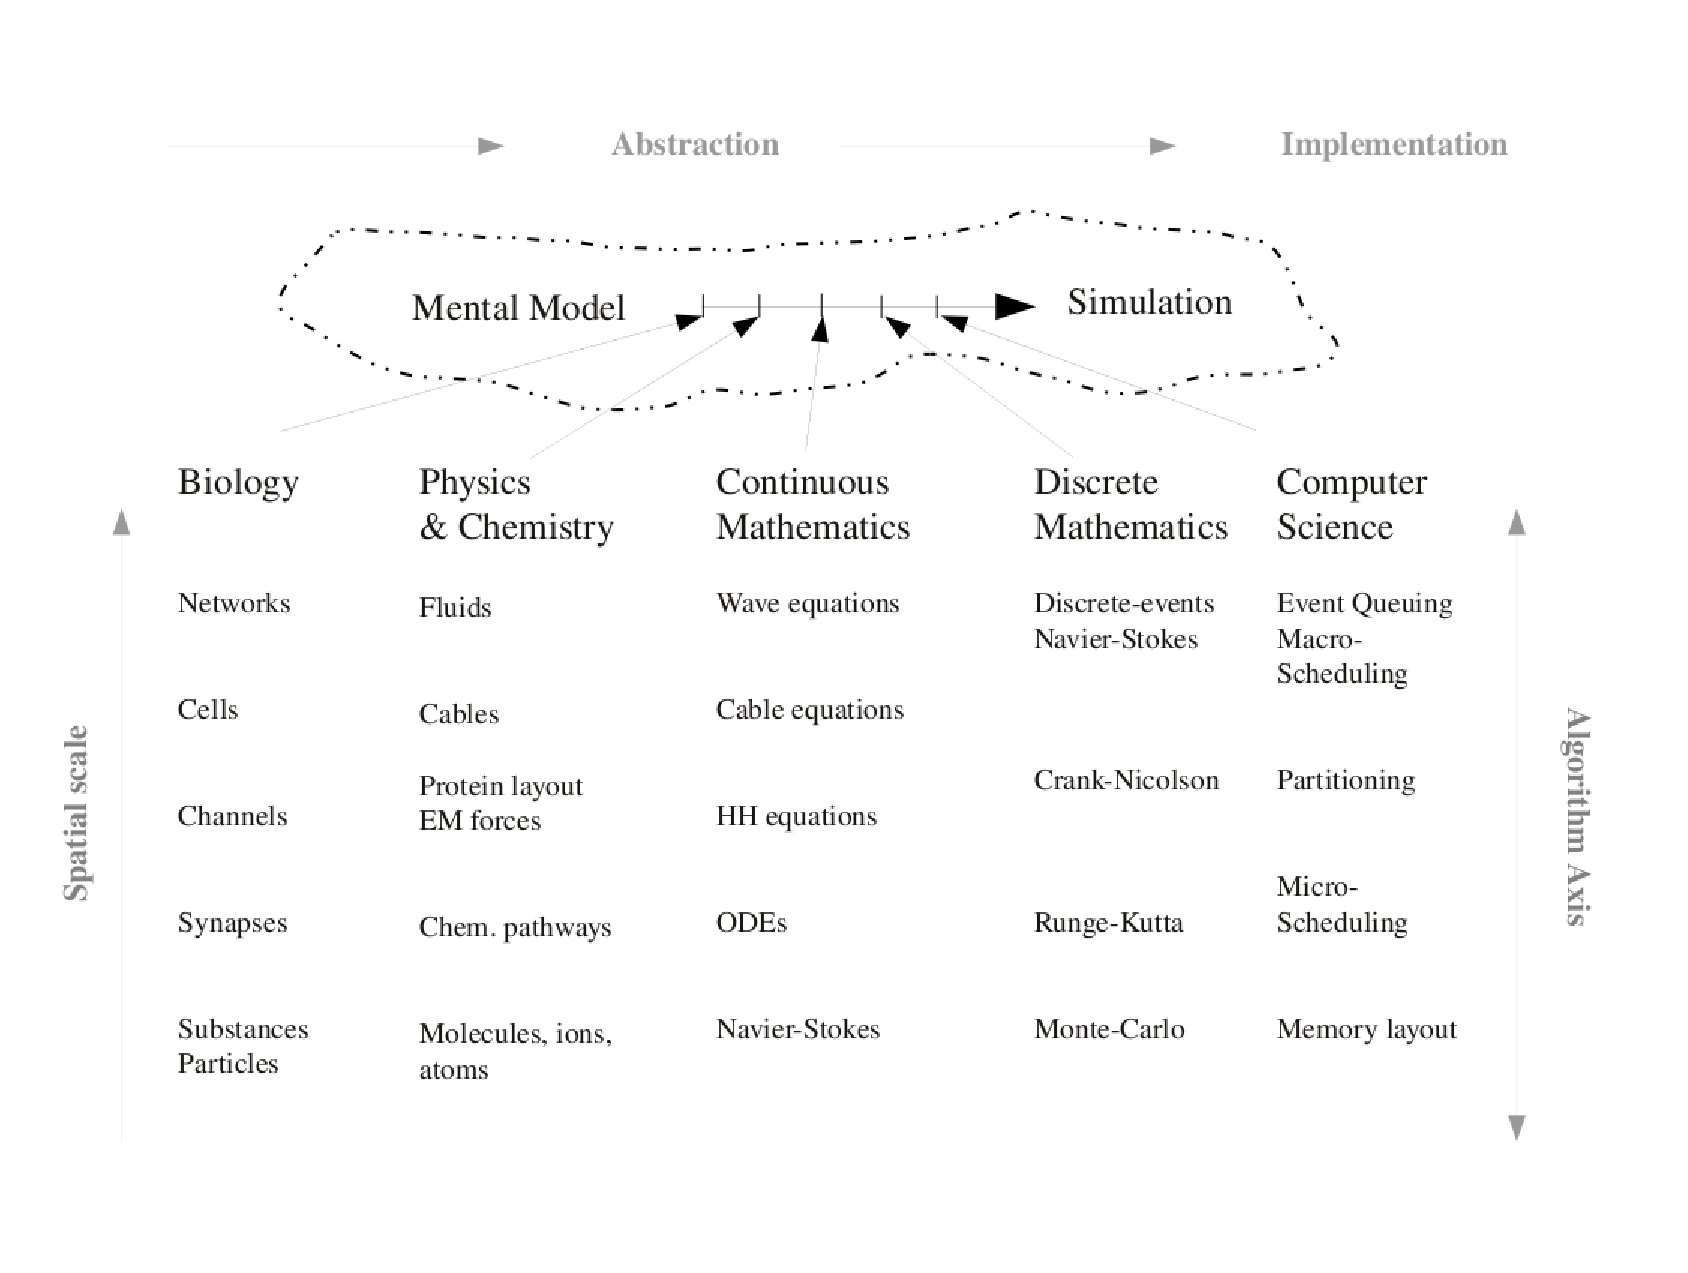
\includegraphics[width=4in]{figures/NS-abstraction-implementation.eps}
  \end{center}
  \caption{ {\bf A Multi-Scale Path from Mental Model to Simulation.} }
  \label{fig:mental-model-simulation-path}
\end{figure}

Each step in the cognitive workflow can be expanded into a matrix where columns span the range of structural detail available for simulation. As an example, Figure \ref{fig:multi-scale-taxonomy} expands the Biology step of the cognitive workflow to give a matrix describing a taxonomy of possible models. Each row illustrates a set of models that spans the range of model detail available at the given level of structural detail. The other steps in the cognitive workflow can similarly be expanded to collectively give a comprehensive framework for multi-scale modelling.

\begin{figure}[h!t]
  \begin{center}
    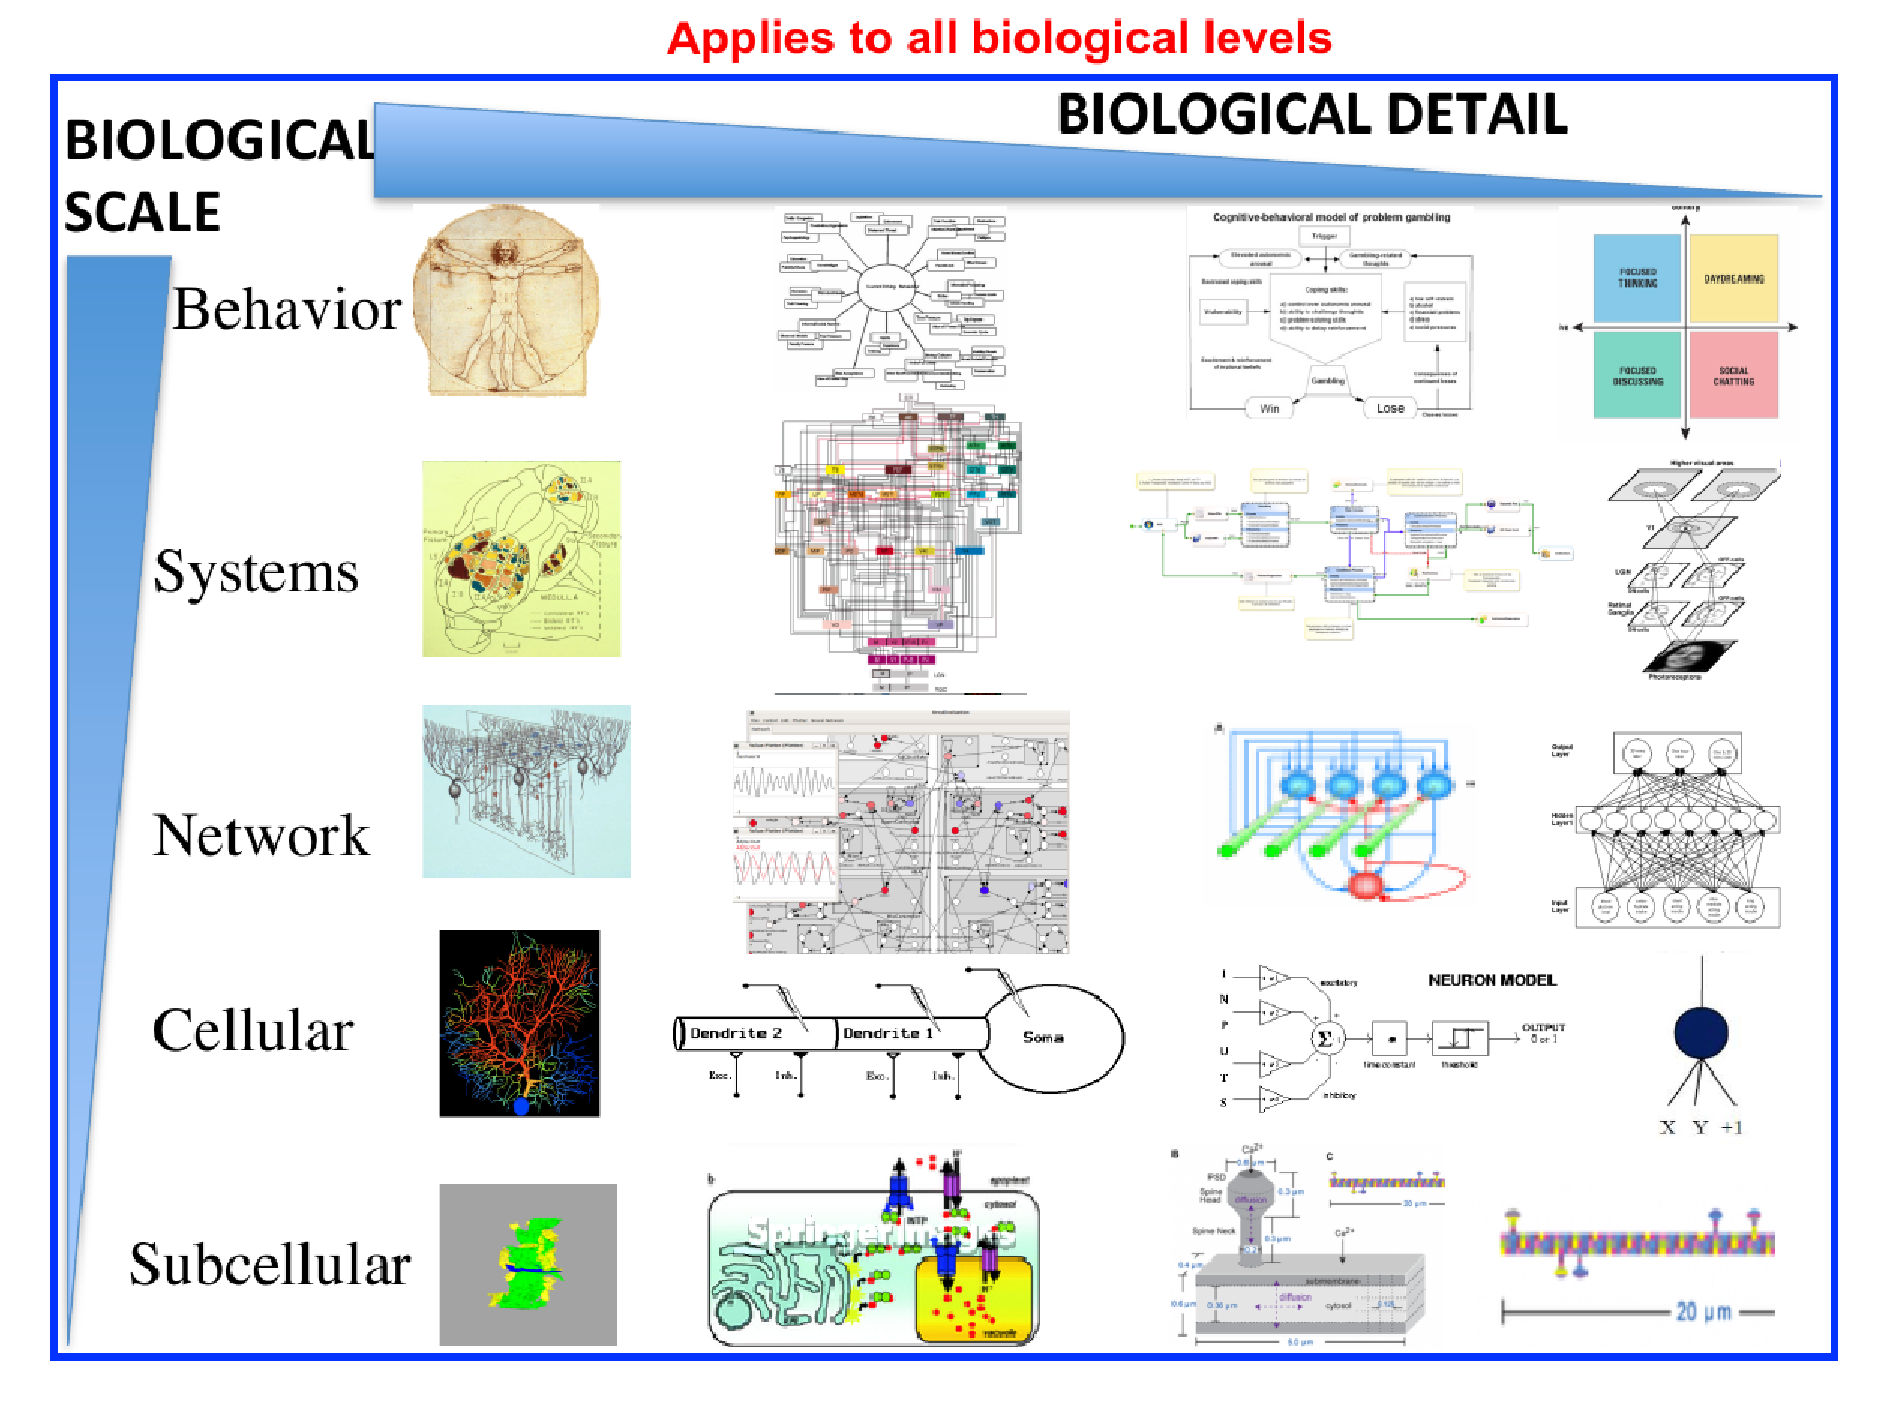
\includegraphics[width=4in]{figures/multi-scale-taxonomy.eps}
  \end{center}
  \caption{ {\bf A Multi-Scale Model Taxonomy.} }
  \label{fig:multi-scale-taxonomy}
\end{figure}

The multidimensional framework implied by Figures \ref{fig:mental-model-simulation-path} and \ref{fig:multi-scale-taxonomy} is based on the relationships between the schemas outlined by Marr, Churchland, and Sejnowski and the user and cognitive workflows described here. We use these relationships to develop a novel and simplifying approach to the simulation of multi-scale models. 

If it is accepted that: (1) a scale specific approximation can be abstracted at each level of a system and disjointly partitioned from its environment \cite{Bertalanffy:1973zr, Heylighen:2006vn}, and (2) the biological levels listed in Figure \ref{fig:mental-model-simulation-path} are plausible, then it is apparent that a realistic neuron model comprised of at least a soma and dendrites, that includes channels and synapses, is a multi-level model simulated at multiple scales. 

We describe the features  of the reconfigured GENESIS simulator (G-3--http://genesis-sim.org) relevant for multi-scale simulation. Together with several scripting examples, we show how primary components of G-3 transparently support multi-scale simulation at the biological levels of networks, cells, channels, and synapses (see Fig. \ref{fig:mental-model-simulation-path}).

%\newpage
%
%Since the 19th century, two groundbreaking discoveries have guided exploration of nervous system function \cite{Churchland:1992uq}: (1) macro effects displayed by nervous systems are dependent on individual cells with axons and dendrites [ref], and (2) these cells can essentially be modelled as electrical devices [ref]. Consequently, the working hypothesis for computational neuroscience has become that emergent properties are high level effects dependent on lower level phenomena in some systematic way \cite{Churchland:1992uq}, with the ultimate research goal considered to be an explanation of how electrical and chemical signals are used to represent and process information \cite{Sejnowski:1988fk}.
%
%Over the last 30 years several axioms have been employed to guide investigators in this endeavour. They include, (1) Level of analysis: Three independent top-down levels have been proposed \cite{Marr:19821kx}: (a) computational theory--what does the system do or what problems does it solve?, (b) representation and algorithm--how does the system solve the problem?, and (c) hardware implementation--how is the system physically realized?, (2) Level of processing: For example, the visual system has roughly hierarchical, reciprocally connected levels of primary processing that fan out upon reaching the level of the cortex, and (3) Level of structural organization: Here, seven broad levels have been proposed \cite{Churchland:1992uq}: (a) systems, (b) topographic maps, (c) layers and columns, (d) local networks, (e) neurons, (f) synapses, and (g) molecules. This complexity\marginpar{what complexity?} has resulted in two propositions \cite{Sejnowski:1988fk}: (1) Because of the the many different structural levels of organization and the fact that models rarely span more than two levels, more comprehensive understanding will require many different types of model, and (2) Intermediate level models must necessarily simplify with respect to the structural properties of lower level elements, but ought to attempt to incorporate as many of the given level's functional properties as actually figure\marginpar{figure?} in the higher level's computational tasks. This approach has led to the development of both realistic\marginpar{one more clarifying sentence needed?} and simplifying brain models that define the end points of a continuum, although any given model may have features of both \cite{Sejnowski:1988fk}.
%
%With hindsight, it is clear that the research paradigm outlined above is firmly located within the traditional scientific method, one that is based on the gathering of complete information about a given phenomenon. Historically, biology in general, and computational neuroscience in particular, has adopted this mechanistic or `Newtonion' view due to its compelling simplicity, coherence, and common-sense \cite{Heylighen:2006vn}. In this view, our knowledge is an imperfect reflection of particular external arrangements of matter. The task of science is to make the mapping or correspondence between external material objects and the internal or subjective cognitive elements\marginpar{maybe use the word 'model' here?} (concepts or symbols) that represent them as accurately as possible. This is achieved through experimentation, where information about external phenomena is collected and arranged to incrementally develop the evolving internal model. Ideally, this should lead to a comprehensive narrative that perfectly describes external reality. This in turn allows accurate prediction of all similar phenomena \cite{Turchin:1990ys}.
%
%Following the development of systems theory (see \cite{Bertalanffy:1973zr}), this view has been challenged. In contrast with the elements of Newtonian ontology (matter, the absolute space and time in which that matter moves, and the forces or natural laws that govern movement), living systems are now considered to be intrinsically open\marginpar{the term 'closed' has not been coined yet}, as they must interact with their environment and cycle matter and energy to maintain metobolism and remain alive. The predictive success of Newtonian models has primarily been due to their focus on closed systems, whereas, open systems depend on an environment much larger and more complex than the system itself, so that its effect can never be truly controlled or predicted \cite{Heylighen:2006vn}. Regularity or organization is not a given, but emerges dynamically out of conflicting forces and random fluctuations, a process aptly described as ``order out of chaos'' \cite{Prigogine:1984ve}.
%
%We now summarize recent developments in the definition of a multi-scale\marginpar{not defined yet} system. Such a system is defined as a collection of properties and relationships that exhibit an essential duality \cite{Heylighen:2006vn}. It is simultaneously both a whole and a part of a more expansive whole or `holon' \cite{Koestler:1990ly}, i.e. there is a cohesion to the parts that allows them to be treated as a whole; and that whole itself is part of the system's environment.
%
%There are at least two fundamental reasons why is is not possible to conceptualize a system defined in this way\marginpar{which way?}: (1) It is only humanly possible to conceptualize at specific scales, not with combinations of conceptualizations at multiple scales, and (2) It is not humanly possible to conceptualize properties separately when they are parts of a system as they are always parts `of' something.
%
%At any scale of conceptualization, properties are always aggregated at least as simple objects and a system at any scale of conceptualization is an approximation or loose congruence of the actual system. A scale specific conceptualization of a system is partial if there are patterns pertinent to an observer's interest in a system that are only available at other scales (where patterns are simple objects, relationships, and their aggregations). This is not an `abstraction' of the system as this means leaving things out with the understanding that what is left out can always be reinserted. What is ``left out'' of a scale specific conceptualization of a system are patterns that might be available at other scales. Such patterns cannot be returned to a scale specific approximation of a system, regardless of resolution or field of view. The `missing' content has no place in the conceptualization as it was never available to it in the first place\marginpar{needs more clarification?}.f
%
%A scale specific approximation of a system can, however, be abstracted at each scale and can be disjointly partitioned from its environment. This means that the whole of the system (as a holon) has a well defined boundary with its environment. To say that a boundary disjointly partitions the approximation of a system from its environment means that simple objects in the conceptualization belong either to the scale specific approximation of the system or to its environment. They can never belong to both\marginpar{is this defining 'open' and 'closed'?}.
%
%Such a boundary, however, will appear inappropriate or even non-existent at other scales of conceptualization. This is because objects (as aggregations of properties and possibly relationships) can be aggregated differently at different scales. This is true even in the unlikely event that the same properties are aggregated at a new scale. Thus, objects that were the basis of the boundary at the first scale are no longer apparent at a second scale. In other words, systems that require multiple scales of conceptualization to properly be understood also have ambiguous or shifting boundaries relative to their environment at the different scales\marginpar{this justifies multi-scale modeling?}.
%
%Regardless of the number of scales used to conceptualize a system, it is not possible to know whether the system has been completely conceptualized. This is a consequence of changing scales which adds, deletes, and reconfigures patterns that are the content of conceptualizations, but there is no way to know or learn that all patterns have been conceptualized at one or more scales, as completeness is not possible. Nevertheless, the use of multiple scales of conceptualization can be understood as a way to asymptotically approach completeness.
%
%Systems theory shows the futility\marginpar{to strong and upsetting to some?} of the Newtonian analytic approach for understanding the living biological material of interest to neuroscientists. That is, to understand any complex phenomenon, it must be taken apart and reduced to its individual components. If these are still too complex, analysis must be taken one step further, and the resulting components studied. If this subdivision is continued sufficiently, the smallest possible part will eventually be obtained\marginpar{this 'definition' should occur earlier in the text}. However, there is no guarantee that it will also be the simplest part. 
%
%According to the principles of systems theoretic analysis outlined above, it is clear there are numerous phenomenological approaches to the development of multi-scale models suited to the transformation of a mental model into a computational simulation. Figure\,\ref{fig:mental-model-simulation-path} illustrates a selection of some of the possible steps, levels, and components of this process. Interestingly, from this perspective, two possible multi-scale models have been in widespread use but not generally recognized for their multi-scale characteristics. One is: (1) Biologically inspired, e.g. a model is specified as a network and a population of detailed channel models, the other (2) Mathematically inspired, e.g. use continuous cable equations to model a neuron, discrete event models for axonal propagation, and Hodgkin-Huxley equations for the channels.
%
%We note that because the multi-scale nature of realistic neuron models was not originally fully appreciated, first generation simulators did not appropriately reflect or incorporate the three essential levels (computational theory, representation and algorithm, and hardware implementation) originally proposed by Marr \cite{Marr:19821kx}. The outcome was a family of first generation simulators that were monolithic and entirely unsuited for the integration of new functionality, which now can be seen to actually be software support for the extension of novel multi-level functionality into a simulator\marginpar{one sentence, two statements, difficult to understand}.
%
%We further note that there is a plethora of so-called second generation simulators that remain primarily focused on the biological and mathematical aspects of multi-scale modelling. It is likely that because they did not incorporate all three of Marr's levels, the progress that might otherwise be expected from a completely configured multi-scale simulator was greatly reduced. Following the recent reconfiguration of the GENESIS simulator it is now clear that it is necessary\marginpar{becomes possible instead of 'is necessary'?} to incorporate Marr's third level or `hardware', i.e. software functionality, to give a comprehensive multi-scale simulator.
%
%On this basis, the third element of a well configured multi-scale simulator is: (3) Software definition. In the remainder if this paper we introduce and describe this ``third leg'' necessary for the construction of an extendable, fully functional, multi-scale simulator. It is based on the Computational Biology Federated Software Architecture (CBI architecture). In this approach, it is the implementation
%of a model for simulation or otherwise, that is contained by a single
%software entity (in this case a single `model-container') that employs the solvers necessary to
%implement different mathematical tools and that communicate with each other at run-time using a communication infrastructure
%provided by the CBI architecture
%(Fig.~\ref{fig:mental-model-simulation-path}).

\section{Methods}

%\subsection{The User Workflow}
%
%The term {\it user workflow} \cite{10.1371/journal.pone.0028956} is
%employed to describe the sequence of necessary steps typically
%employed by a person in developing a computational model and employing
%simulation to generate data for subsequent analysis. In this sense it
%is a depiction of a sequence of operations, declared as the work of a
%person or a group of persons \cite{Belhajjame:2001fv}.
%
%A comprehensive user workflow can be employed to guide the separation
%of the different aspects of a model by organizing user actions into
%different categories during model development.  The workflow allows
%distinctions to be made between an object under investigation, the
%tools used to perform the investigation, and the operations performed
%during the investigation. It also distinguishes between the results
%obtained from a single investigation and the method used to define
%multiple investigations in a series. The user workflow identifies five
%steps in total (explained in more detail in Results).
%
%\subsubsection{The Ideal User Workflow for Simulations in Neurobiology}
%
%As many more data flows can exist than are present in reality, each actual
%data flow can be considered in the context of a sequence of user
%actions or workflow. We define an ``ideal user workflow'' that provides a canonical form
%of a user workflow specific for neural simulators. In this section, we introduce
%the set of typical workflows that use CBI simulator architecture
%applications by describing the ideal user workflow where a user wants to model a biological system. We then briefly mention a second set of workflows that comprise user extensions of the
%functionality of an implementation of the CBI architecture. Both sets of workflows are presented in a technology and implementation free manner.
%
%%In this paper we discuss the first set of workflows by introducing an
%%and we superficially touch upon the second
%%set of workflows.  All workflows described in the following sections
%%are technology and implementation free.
%%Examples are given for
%%purpose of illustrating the meaning of the text, and neither for
%%illustrating the current (state of the existing) implementation, nor
%%for a possible implementation in a specific technology.
%
%A five step outline of an ideal user workflow for the development,
%implementation, and simulation of a computational model has been
%identified from the workflow of users of the GENESIS neural simulation
%platform \cite{cornelis02:_tutor}.  Importantly, the workflow
%explicitly distinguishes between the static structure of a model of
%the biology (Step 1), the dynamic state of its simulation (Step 3),
%and the analysis of this dynamic state (Step 4). We also note that
%this workflow does not specify any particular order for its
%completion. However, for any given case, meaningful simulation output
%will only occur with completion of Steps 1--4.
%
%\subsubsection{Step 1: Construct Model}
%
%The simulator shell and the graphical user interface (GUI) each
%provide an interface that interprets user input such that the
%simulator `understands' different commands and performs the
%appropriate actions. Simple models can be created directly within the
%simulator shell by entering a sequence of commands. More complex
%models are available to the shell from libraries or databases external
%to the simulator. Shell tools can then be used to explore and check
%the integrity of a model. Following any necessary or desired changes,
%a new version of the model can be saved.
%
%\subsubsection{Step 2: Design Experiment}
%
%Specific change management tools can be used to make small
%modification to a model, e.g. to set model parameter values specific
%to a given simulation.  Configuration tools support the definition of
%the stimulus or activation parameters for a given simulation run or
%experiment and the output variables to be stored for subsequent
%analysis by independent software.
%
%\subsubsection{Step 3: Run Simulation}
%
%Shell tools can be used to check the state of a given simulation or reset the simulation time step and solved variables to their initial values. After a simulation is run, output values are flushed to raw result storage for subsequent data analysis. The model state can be saved at any simulation time step. This allows it to be imported into a subsequent simulator session for further development and exploration.
%
%\subsubsection{Step 4: Process Output}
%
%The validity and location of simulator output is checked prior to data
%analysis. Output can be analyzed either within the simulator or piped
%to external applications such as
%Matlab. % for subsequent data analysis.
%
%\subsubsection{Step 5: Iterate}
%
%A modeling project is established by the introduction of iterators
%into the user workflow. Iterators close the loop between the output of
%results and model construction, they include: Automated construction
%of simulations and batch files, static parameter searching, and active
%parameter searching using, for example, dynamic clamp technology.
%
%
%\subsection{Principal Concerns}
%
%In software engineering, the process of partitioning a program into
%logical functions that minimize overlap is referred to as a
%{\it separation of concerns}.  We consider that a principled separation of concerns is a prerequisite
%for the development of advanced computational modeling techniques in
%the neurosciences. User {\it concerns} have a direct influence on the
%user's experience of an application.  Technical concerns have a clear
%and direct influence on the partitioning of a program into its primary
%functional blocks, and are also crucial for problem diagnosis and
%guaranteeing the correct behavior of software.  Here, we propose there
%are two principal concerns that underly the development of modeling
%software: (1) Separation between data and control, and (2) Separation of biology and mathematics through the use of data-layering.
%
%\subsubsection{Control versus data}
%\label{sec:data-vs-control}
%
%All software can be understood in terms of algorithms operating on
%input data to produce output data. For experimental research, the
%natural distinction between data and algorithms can be compared to the
%distinction between the biological system (data to be investigated)
%and the stimulation paradigm (tools supporting data investigation).
%For computational research, the distinction between data and
%algorithms leads to a separation between model (data) and simulation
%control (control of data flows).
%
%\subsubsection{The requirement for data-layering}
%\label{sec:data-layering}
%
%%For example, at the biological level,
%%a dendritic spine is considered to be a single morphological entity
%%but its mathematical equivalent is commonly described by a circuit
%%composed of two cable equations: one for the head and one for the
%%neck. Similarly, many empirical advances have been made in our
%%understanding of the electrophysiological role played by intracellular
%%calcium. However, this has frequently been at the expense of
%%conflating calcium channel activity with intracellular calcium
%%concentrations which, computationally, are at least two distinct
%%components of a realistic model. An important consequence is that the
%%development of an optimized simulation can be a significant challenge
%%for the neuroscientist unfamiliar with mathematical and computational
%%theory.
%
%It is the capacity to represent a model in terms of
%biological concepts such as neuron, dendrite, soma, channels, and molecules, that
%allows a user to clearly relate a model to the original scientific
%questions.  One way to achieve this goal is to separate the high-level
%biological representation of a model from its low-level mathematical
%implementation and provide operators that convert between them.
%This insulates the process of model construction
%from the computations performed during a simulation. 
%
%The relationships between simulator control and data modules in a federated architecture are symbolized by the horizontal arrows in Figure~\ref{fig:data-control}, whereas the relationship between high level biological concepts and their mathematical implementation are symbolized by the vertical arrows. It is the separation of the principle concerns along the horizontal and vertical axes that allows independent modules to be designed. This process underlies the
%construction of a simulator composed of stand-alone
%{\it component}s and forms the basic meta-framework
%referred to as the CBI architecture.
%
%Importantly, we note that a simulator can be efficiently modularized
%when only horizontal or vertical interactions are allowed between the
%modules illustrated in Figure~\ref{fig:data-control}. The larger the
%number of interactions allowed between diagonally located components,
%the more difficult it becomes to functionally separate simulator
%components and to maintain and extend the
%resulting software application. Diagonal interactions are forbidden in the CBI architecture as they foster the mixing of functionality across different levels that ultimately leads to the creation of monolithic software applications.
%
%%The first implementation of the CBI architecture has been that of  G-3. We use this software platform to present an overview of the CBI federated software architecture through the example of the the new G-3 simulator. In doing this we follow the ideal simulator workflow presented in Methods.
%
%% Figure 2
%% \noindent {\bf Place Figure \ref{fig:data-control} about here.}
%
%\begin{figure}[ht]
%\begin{center}
%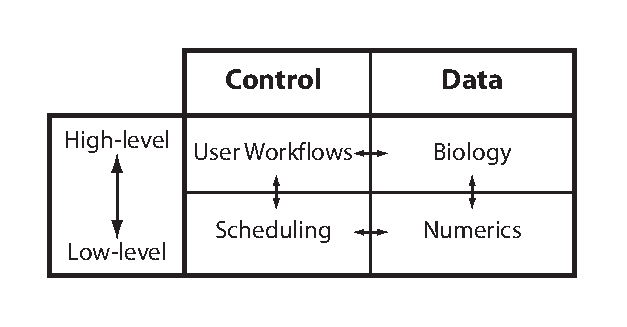
\includegraphics[width=4in]{figures/matrix.eps}
%\end{center}
%\caption{ {\bf Principle concerns.}  The four fundamental building
%  blocks of a simulator are distinguished by separating (i) Data from
%  control, and (ii) High level biological concepts from their
%  mathematical implementation. In a federated architecture the only
%  allowed interactions between modules are those indicated by the
%  vertical and horizontal arrows. Diagonal interactions are forbidden
%  as they ultimately lead to interactions that result in the existence
%  of a monolithic software architecture.
%}
%\label{fig:data-control}
%\end{figure}
%
%
%\subsection{Separation of Concerns}
%
%Consideration of the principal concerns of data, control, and data layering were used to expand Figure~\ref{fig:data-control} by the separation of concerns principle. This key principle in software engineering states that a given problem involves different kinds of concerns. To cope with complexity, these concerns should be identified and separated \cite{Dijkstra:1982fu}. The aim is to achieve engineering quality factors such as robustness, adaptability, maintainability, and reusability.  Ultimately, this results in clear model scripts where the biological aspects of a model are separated from the peripheral code that implements a model during a simulation.
%
%% Dijkstra EW (1982) On the role of scientific thought. in Dijkstra, Edsger W.. Selected writings on Computing: A Personal Perspective. New York, NY, USA: Springer-Verlag New York, Inc. pp. 60�66.
%
%In this section we present the outcome of a separation of concerns based on the principal concerns of data- and control-related simulator components introduced above. Initially, the biological and numeric representations and user workflows and scheduling modules are expanded to give the principal functions of the CBI architecture.
%
%Our analysis generated the primary functions of the CBI architecture illustrated in Figure~\ref{fig:cbi-architecture-simple}. The mechanism identified for separation of model construction from the low level computations performed during a simulation was the addition of a mid-level software layer. This intermediate layer provides function and data bindings between scripting applications and database interfaces, respectively, and the low-level back-ends. Note, this figure maintains the relationships between the four principal concerns identified in Figure~\ref{fig:data-control} by separating high level biological representations (Fig.~\ref{fig:cbi-architecture-simple}A) and low level mathematical implementation (Fig.~\ref{fig:cbi-architecture-simple}B), as well as separating control functions from data streams. Note also, the addition of a GUI to connect high level scripting applications with database interfaces.
%
%\subsubsection{User Workflows and Biological Data}
%
%%Many more possible data flows exist than there are present in reality. So each data flow must be considered in the context of a sequence of user actions or workflow. Initially, the focus is on regular workflows using CBI simulator architecture applications, e. g. where a user wants to model a biological system. We then briefly mention other workflows that support user extensions of the functionality of an implementation of the architecture.
%%
%The first step in our ideal user workflow involves creating or
%importing a model. It maps directly to high-level biological
%representations via a simulator shell or GUI.
%%Similarly the second
%%step in the ideal user workflow allows for the construction and
%%management of high-level representations of experimental protocols and
%%the physical objects used to implement them.
%This interface
%straddles the Control/Data divide and replaces the upper horizontal
%arrow connecting the {\tt User Workflow} and {\tt Biology} modules in
%Figure~\ref{fig:data-control}. It enables the workflow by assisting
%either the development of simple cell models from the command line of
%a simulator shell via the {\tt Scripting Libraries \& Applications}
%module or the importation of model descriptions via the
%{\tt Database Interfaces} module (see
%Fig.~\ref{fig:cbi-architecture-simple}).
%% File formats currently recognized include SWC, the GENESIS P format, the declarative NDF file format, and once finalized, the NeuroML model specification format.
%
%Step 2 of the ideal user workflow typically requires biological
%expertise to design an experiment.  This includes the definition of
%constants such as the command voltage of a voltage clamp protocol,
%delays and duration of a current injection protocol, and model and
%simulation inputs and outputs.
%
%%For example given a
%%morphology, what are the total surface and volume of the cell, convert
%%it to a model, apply current injection into the soma, and record the
%%response from a distal dendrite.
%
%\subsubsection{Numerics and Scheduling}
%
%Step 3 of the ideal user workflow deals with the checking,
%resetting, and running of a simulation.  This is accomplished via the
%{\tt Function Bindings} module of the CBI architecture (see
%Fig.~\ref{fig:cbi-architecture-simple}).
%%This module provides a
%%mid-level software layer that separates the high level biological
%%implementation from the low level numerical implementation of a model
%%by providing translators that are capable of making intelligent
%%decisions about mapping the given biology to the required numerics.
%
%At a technical level the simulation involves scheduling mathematical
%operations on, and communication of, the numerical representations of a
%biological model.  This step is indicated by the horizontal arrow
%between {\tt Scheduling} and {\tt Numerics} in Figure~\ref{fig:data-control} and
%is encompassed by the {\tt Controllers \& Communication} and {\tt Solvers}
%modules illustrated in Figure~\ref{fig:cbi-architecture-simple}.
%
%Elaborate user workflows can stop and restart running simulations and
%provide new inputs to a model thereby imposing high-level control on
%the low-level back-ends via the controller.

%\subsection{The CBI Meta-Framework for Simulator Development in Neurobiology}

%\subsubsection{Overall Design Objectives}

%During development of the Computational Biology Federated Software
%Architecture (CBI architecture), several important objectives emerged
%from a separation of concerns.  They were used as a guide for the
%design of this next generation neuronal simulation engine and
%included: (1) Reduced complexity of software modules when compared to
%a monolithic system, (2) Simplified documentation of modules in terms
%of inputs and outputs, (3) Easy incorporation or removal of individual
%modules as required, (4) Simplified development and testing of modules
%as stand alone components, and (5) Clear delineation of scope for new
%module development.

\subsection{Structural Overview of the CBI Architecture}

The Computational Biology Initiative Federated Software Architecture (CBI architecture) is defined as a modular paradigm that places
stand-alone software components into a set of logical relationships \cite{10.1371/journal.pone.0028956}.
In doing so, it defines a modular framework that provides the
necessary parts of a simulator. The architecture takes its name from the Computational Biology Initiative at the University of Texas at San Antonio, where development was first initiated.

A schema identified by separation of concerns (see
 \cite{10.1371/journal.pone.0028956} for details) is expanded in
Figure~\ref{fig:cbi-architecture-simple} to give the modules that
form the building blocks of the CBI architecture.  The schema retains
the four quadrants of simulator functionality identified by the
separation of concerns, including separation between control and data 
and the notions of high-level representations for biology and low-level data for
numerics (Fig.~\ref{fig:cbi-architecture-simple}: indicated by vertical and
horizontal dashed lines, respectively).

We note that the integrity of the simulator is maintained by only allowing interactions between vertically and horizontally located modules. Diagonal interactions are forbidden as they foster the mixing of functionality across different levels and typically lead to monolithic software applications. Ultimately, it is this partitioning of simulator functionality that lies at the core of simulator extensibility and provides the architectural foundation for transparent multi-scale simulation.

\begin{figure}[ht]
\begin{center}
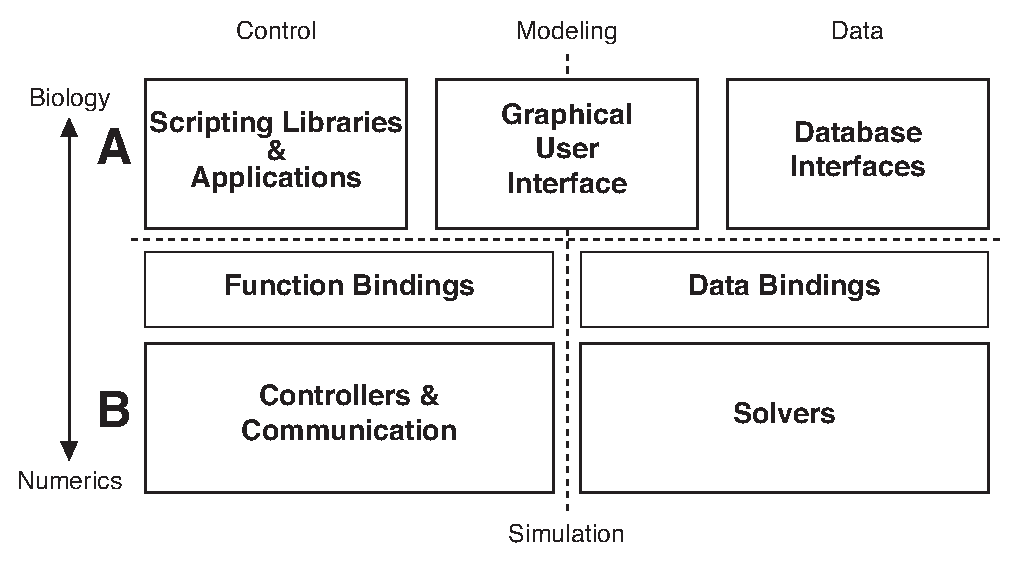
\includegraphics[width=4in]{figures/cbi-architecture-simple.eps}
\end{center}
\caption{ {\bf Overview of a federated software architecture:}
  The primary functional modules defined for
  the CBI federated software architecture are illustrated.  Control modules are given
  to the left and data modules to the right.  A. The top layer
  contains conceptual data and controls representations of the biology
  of a model. B. The bottom layer contains representations that are
  numeric and thus close to the hardware.  The middle or intermediate
  layer bridges between these `biological' and `numerical' layers in a
  CBI compliant simulator. Importantly, Control (Scripting Libraries
  \& Applications) and Data (Database Interfaces) modules can interact
  either directly or via the Graphical User Interface. }
\label{fig:cbi-architecture-simple}
\end{figure}

We refer to the CBI architecture as being `federated' as it extends
the modular approach associated with the development of single
applications to the functional integration of otherwise independent
applications.  Federation aims to provide a unified interface to
diverse applications and ideally make them look like a single
system to the user. In doing so, it provides transparency, heterogeneity, a high
degree of function, autonomy for the underlying federated sources,
extensibility, openness, and the possibility of highly optimized
performance (see \cite{federated-2002-xyz}). Here, extensibility is defined as a system design
principle where an implementation takes into consideration future
developments. An extensible system is one that includes mechanisms for
expanding or enhancing the system with new capabilities without having
to make major changes to system infrastructure. 

Enhanced application interoperability and performance is available
through the use of flexible high-level scripting languages that support
diverse workflows, low-level application programmer interfaces
(API)s, and application binary interfaces (ABI)s (see \cite{Cornelis:2011fk}).

% For completeness, we note that northbound and southbound interfaces
% are indicated in this figure. Northbound interfaces conceptualize
% lower level details, whereas, the southbound interfaces decompose
% the concepts in technical details, which are mostly specific to a
% single component of a software architecture. Northbound interfaces
% normally communicate with southbound interfaces of higher level
% components and vice versa. By convention, north- and southbound
% interfaces are drawn at the top and bottom of an architectural
% overview, respectively.

In summary, the CBI architecture provides a template for software
development that, at its core, contains a simulator.  Additionally,
the modularity and layering of the architecture simplifies connection
to independent applications related to model construction
and instantiation and the analysis and display of simulation output.

\subsubsection{Behavioural View of the CBI Architecture}

Figure \ref{fig:cbi-architecture-expanded} expands Figure \ref{fig:cbi-architecture-simple} to give more
detail of the structural relationships between the different modules and
sub-modules of the CBI architecture (previously described in \cite{10.1371/journal.pone.0028956}). The behavior of
the CBI architecture is defined by the functional and dynamic
connectivity provided by these individual modules. This behavior is now introduced within the context of the user workflow.

\begin{figure}[h!t]
  \begin{center}
    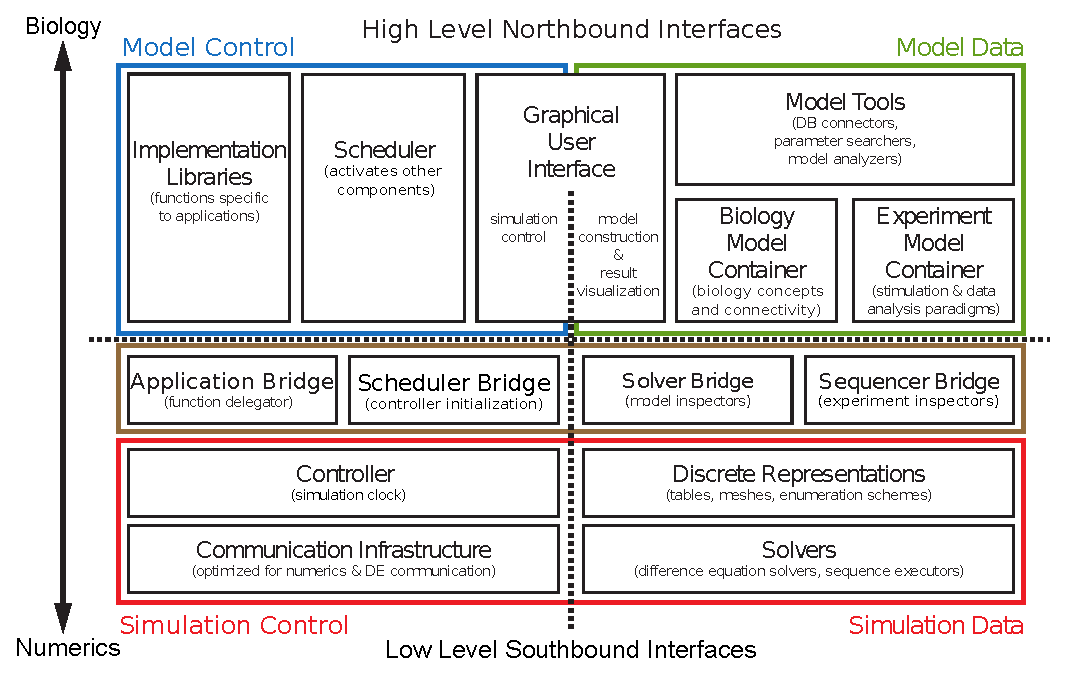
\includegraphics[width=3.33in]{figures/cbi-architecture-expanded.eps}
  \end{center}
  \caption{ {\bf Detailed view of the Computational Biology Initiative
      federated software architecture.} Relationships of sub-modules
    within each of the primary functional modules given in Figure
    \ref{fig:cbi-architecture-simple} are illustrated.  North bound interfaces group
    and conceptualize the details of the modules and interact with
    south bound interfaces of higher level modules.  Steps 1--3 of the
    user workflow induce data cycling between the
    upper layers (blue and green boxes) and lower layers (red box).
    Ultimately, the two layers interact to implement a single simulation.
    By design, any type of model including multi-scale models will
    exhibit this data cycle. In contrast to previous versions of GENESIS and
    other neuronal simulation platforms, the design of G-3 is
    fundamentally modular, separating different functional components
    of the simulator into their own modules. Importantly, G-3
    separates model descriptions from their mathematical representations.  This simplifies the
    implementation of new {\bf Solvers} and other run-time software
    components. The communication infrastructure connects different
    {\bf Solvers} to simulate different parts of a model and can `upscale' or `downscale'
    numerical data as needed. Additional detail is given in \cite{10.1371/journal.pone.0028956}.}
  \label{fig:cbi-architecture-expanded}
\end{figure}

%\subsubsection{Data-flows in the CBI Architecture}
%A (G)UI translates user actions into a family of events that propagate
%to other components of a software architecture, impact the internal
%states of these components, and direct the data flows between them.
%In the CBI architecture each software component is specialised in
%implementing one particular function and performs the defined
%operations on the data it is passed.
%A functional architecture is an overview of a software system that
%identifies the global functions of the system.  These functions define
%the scope for experts for improvement of the system as a whole.  The
%CBI architecture is structured according to low-level vs. high-level
%functions in the system complemented by the data and control
%functions.  As a consequence, a feature of the CBI architecture is
%that rich data flows occur between software components, but not
%necessarily within them.
During the phase of model construction prior to simulation, users
combine models from files and databases.  When the simulation runs,
the numerical {\bf Solvers} perform the calculations of a simulation,
and save the output back to files and databases.  When these two steps
are combined they imply a cyclic data flow from files and databases to
the {\bf Solvers}.
%  Here we explain how user actions and data flows
%relate to one another in the CBI architecture and define the overall
%behavior of an implemented
%software system.\\

In more detail, as a result of Steps 1--3 of the user workflow (construct model, design experiment, run simulation), data flows both through and between software components. The cycle described here is for a single neuron simulation, however, all scales of model will exhibit similar activity.

Once Step 3 is completed, data generated by dynamic states of the model are available through databases and files. Consequently, there is no requirement to query software components that deal with numerical data. This provides an operational barrier to assist with preventing incremental conversion of a CBI compliant simulator to its monolithic equivalent.

In Step 4 of the user workflow (output), while maintaining the integrity of the separation of concerns, the availability of any model data from the {\bf Biology\,Model\,Container} and the functionality of {\bf Scripting\,Libraries\,\&\,Applications} can be used to connect the CBI architecture to external tools, for example Matlab (to implement output analysis).

At Step 5 of the user workflow (iterate), simulation output data and model parameters and structure available in the model containers can be combined, for example, to provide automated script generators for the creation of batch simulations. Importantly, at this stage of the workflow, the back-ends of the CBI architecture (indicated below the dotted horizontal line in Figures \ref{fig:cbi-architecture-simple} and \ref{fig:cbi-architecture-expanded}) are unavailable. 

%Intermediate results may be analyzed or aggregated by
%analysis libraries, e.g. for signal analysis and binning of spikes.
%These libraries are accessible to the CBI architecture from the {\tt
%  Scripting Libraries \& Applications} software component.

%\paragraph{Running a Single Cell Model:}

%When a user wants to learn more about the electrophysiology of an
%existing cell model, it must be instantiated, the stimulation and
%output protocols configured, the simulation run, and the results
%interpreted.

%In Step 1 of the user workflow, the GUI is opened and a cell
%model is selected from a database listing of available models.
%Internally, model selection is translated into an event that instructs
%the {\tt Biology Model Container} to load a selected model from a
%database and store it in memory using data structures for efficient
%storage and retrieval by other modules.  During initial inquiry, a
%user may typically be interested in derived model parameters such as
%the total surface area of a neuron, with and without spine correction,
%while a sophisticated GUI can also present a table of the channels
%employed in the model along with their conductance densities and
%reversal potentials.  More dedicated queries related to specific brain
%areas or neuron types are supported by the {\tt
%  Scripting Libraries \& Applications} module.

%%A model can be queried in this way when it is stored by
%%the {\tt Biology Model Container}.

%A typical example of Step 2 of the ideal user workflow is the design
%of an experiment that applies current injection pulses to a neuron's
%soma and defines simulation output as the somatic membrane potential
%and somatic transmembrane currents.  The {\tt
%  Experiment Model Container} stores the definition of the current
%pulse amplitude and duration, which is translated by a {\tt
%  Sequencer Bridge} to a sequence of simulation-time events prior to
%the start of a stimulation.  These events are then executed by the
%{\tt Command Sequence Executor} during a simulation.

%Running the simulation in Step 3 of the ideal user workflow starts
%with the {\tt Biology Model Container} examining a stored model to
%determine model time constants or other parameters that are relevant
%for the accuracy of a numerical simulation.  The {\tt Solvers} then
%fill their data structures with parameter values optimized for
%simulation, for instance a Crank-Nicolson solver can multiply the
%membrane capacitance with the time step during this initialization
%phase instead of at every simulation time
%step \cite{borg-graham00:_addit_effic_comput_branc_nerve_equat}.  For
%this, the memory image of a model must first be expanded into a
%representation that includes the mathematical equations and parameters
%relevant to the given simulation but, for instance, does not include
%the spatial layout of segments as this is not required by the {\tt
%  Solvers}.  (Note: `Segment' is a high level term employed to describe different parts of the biological model of a dendritic morphology. The equivalent low level (computational) term is `compartment'. It refers to the numerical representation of a segment.) This behavior is different from that of existing
%simulators, e.g. GENESIS 2. Such simulators do not make an explicit
%distinction between internal data structures for model representation
%and data structures for computation.  Consequently, they often
%generate redundant data during the initialization of a simulation.

%In network simulations the {\tt Solvers} employ the {\tt
%  Connectivity Translator} to initialize its simulation-time
%communication data structures and to connect to the {\tt
%  Communication Infrastructure}.

%When a user instructs the simulator to start a simulation, for
%instance by pushing a button in a GUI, the {\tt Controller} generates
%a list of instantiated {\tt Solvers}.  It then advances the simulation
%clock and requests each {\tt Solver} to update its internal state.
%The {\tt Communication Infrastructure} connects the {\tt Solvers} for
%efficient communication of the solved variables.  {\tt Solvers} that
%were configured for output, save results to a file.  When the
%simulation finishes, either by user action or following a preset
%simulation period, output buffers are flushed to disk.

%The independence of the {\tt Solvers} in the CBI architecture not only
%allows for better optimized implementations, but also enables
%additional simulator functionality such as serialization of the model
%state to a file.  This allows a simulation to be resumed at a later
%time and reduces the total simulation time of a complex model if it requires
%a calibration phase prior to the application of an experimental
%protocol.

%%During Step 4 the dynamic state of the model is available from the files and databases for further analysis.

%% Steps 4 and 5 are complementary to Steps 1-3 of the ideal user workflow.

%%The data cycle between databases and files, and the solvers in Steps
%%1-3 of the ideal user workflow results in all simulation simulation output
%%is available through these databases and files.  Once these steps
%%have been completed, the back-ends of the CBI architecture are not
%%available anymore.  The simulation result data can then be combined
%%with the model parameters and structure available in the {\tt
%%  Biology Model Container} through {\tt
%%  Scripting Libraries \& Applications} to implement Step 4 and 5 of
%%our ideal user workflow.

%As a result of Steps 1--3 of the ideal user workflow, data flows both
%through and between software components that conform to a CBI
%architecture: the data cycles between databases and files, and
%back-end {\tt Solver}s.  Here we have described this cycle for a single
%neuron model and, as we briefly noted, it also occurs for network
%models.  By design any type of model including multi-scale models
%will exhibit this data cycle.

%In Steps 4 and 5, the availability of any model data from the {\tt
%  Model Container} and the functionality of {\tt
%  Scripting Libraries \& Applications} can connect the CBI
%architecture with external tools while maintaining the integrity of
%the separation of concerns.
%%The laterality of the software component connectivity activated during Step 4 is not an issue.
%{\tt Scripting Libraries \& Applications} connect to external tools
%such as Matlab to implement output analysis.
%%  Integration, at Step
%%4 of the ideal user workflow, with software platforms such as RTXI
%%make direct interaction with experiment possible.
%They also allow simulation output data to be combined with the model
%parameters and structure available in the {\tt
%  Biology Model Container} to implement Step 5 of our ideal user
%workflow, for instance to provide automated script generators for the
%generation of batch simulations.  Importantly, at this stage of the
%workflow, the back-ends of the CBI architecture (indicated below the dotted
%horizontal line in Figures~\ref{fig:cbi-architecture-simple}
%and~\ref{fig:cbi-architecture-expanded}) are unavailable.  Once Step 3
%is completed, all the data of the dynamic state of the model are
%available through databases and files.  Consequently, there is no
%requirement to query the software components that deal with
%numerical data. This ultimately prevents the implementation of
%diagonal interactions in the software and the creation of a monolithic
%simulator.

%% are technically unrelated to a simulation run and may
%%fall outside the scope of the CBI architecture.  On the other hand
%%{\tt Scripting Libraries \& Applications} may connect to external
%%tools such as Matlab to implement output analysis and include script
%%generators for automation of batch simulations and platforms such as
%%RTXI for a direct connection with experiments.

%%For convenience one could implement a short-cut diagonal into the CBI
%%architecture for implementation of aspects of Steps 4 and 5, and for that matter other Steps, but this ultimately would limit the functional scope of the resulting simulator.

%%All model data is available through the model container and the output (files or databases).  

%%Modules plugged in during Step 4 have access to all data via the model container.

\subsection{GENESIS 3.0}

The software architecture developed for G-3 supports a capacity for federated and modular software development that directly enables multi-scale modelling.  Furthermore, its structure also
supports the direct interaction with, or embedding of, models at different
levels of scale.  During model construction this is accomplished
through the reconfiguration of the internal model storage format,
while during simulation run-time it occurs through
specific software modules that create intermediary representations of
variables present at multiple scales (described in more detail below).

Several explicit features of G-3 allow
new software components to be rapidly incorporated into the simulator: (1) modularity of the CBI architecture supports the development of new {\bf Solvers} independently of
other software components. This encourages full focus on the mathematical
aspects of {\bf Solvers} and their implementation and leads to better
optimization, (2) the {\it Developer\,Package} facilitates integration of
new {\bf Solvers} into the build system of G-3 enabling immediate regression
testing, (3) easy extension of the configuration of the internal model
storage format to establish new declarative model tokens and
parameters recognized by new {\bf Solvers}, (4) easy construction of an
interface between the internal data storage format and the core of new
{\bf Solvers}, and finally, (5) a communication
software component that creates simulation run-time interfaces between {\bf Solvers}.

Solvers currently available in G-3, starting at the highest level, include: {\bf DES}, a discrete event queuing and distribution infrastructure for network modelling, {\bf Heccer}, a single neuron solver, {\bf Chemesis-3}, a simple reaction-diffusion system solver, and {\bf Experiment}, which provides simulation-time components for current injections, time-tables, and output.

%\subsubsection{Extending GENESIS-3}

%The G-3 documentation systems describes the procedures used for G-3
%extension.  Extending G-3 can involve the implementation of a new
%solver, or, when the required functionality is tangential to an
%existing solver, it can require source code additions to an
%pre-existing software component.  Here we describe the integration of
%a new solver, ie. the steps followed for the implementation of
%{\bf Chemesis-3}.

%\begin{enumerate}[noitemsep,nolistsep]
%\item The developer package integrates the different software
%  components of G-3.  The definition of a new component ``chemesis3'' in
%  the developer package allows for its smooth integration with other
%  G-3 software components such as the model-container.
%\item The implementation of the core of a new solver is independent of
%  the development of other software components.  This allows full
%  focus on the mathematic aspects of the solver and their
%  implementation.
%\item Optionally, the model-container can be extended with new tokens
%  that are specific to the new solver.  Configuration of the
%  model-container defines the new tokens and their parameters.
%\item An interface must be written between the model-container and the
%  core of the solver.  The model-container defines an API that makes
%  abstraction of the biological structure the model.
%\end{enumerate}

\subsubsection{The Model Containers}

\paragraph{Biology\,Model\,Container}
Provides a solver-independent internal storage
format for models. Stores biological entities and
end-user concepts and annotates the structures and concepts of a
model with biological, physical, and mathematical quantities. By
`containing' the biological model, the {\bf Biology\,Model\,Container}
relieves the implementation of the numerical core of a solver from the
pressure of user-friendly model representation.

Because all model components are interactive parts of a single
model-container \cite{10.1371/journal.pone.0028956}, existing and
new G-3 {\bf Solvers} can be incorporated to simulate different aspects of the
same model.  This {\em scale-linking} functionality of G-3
instantiates dedicated run-time software components that contain
intermediary representations of solved variables able to pass both
{\em upscale} and {\em downscale} values to {\bf Solvers} operating at different
levels of scale.
%  Technically, in the case of {\bf Chemesis-3} and the
%linear cable solver, for example, these modules calculate weighted
%space-time averages.
It is through this computational mechanism that the {\bf Biology\,Model\,Container} 
supports transparent construction and simulation of multi-scale models.

\paragraph{Experiment\,Model\,Container}
Stores a model of a stimulus paradigm and desired output parameters.
It also defines and stores a hierarchical sequence of stimulus-related
actions (e.g. start and stop time of a current injection) and their
dependencies.

Finally, we note that the model containers define models in a purely declarative,
extensible language.

\subsubsection{The Neurospaces Description Format}

The Neurospaces Description Format (NDF) file format developed for the model containers
was originally designed as a file-based user-editable declarative
interface to the {\it hsolve} method used by GENESIS-2
\cite{cornelis03:_neuros}\cite{beeman12:_years_comput_neuros}.
Subsequently, its single neuron modelling functionality was expanded
with network modelling capabilities.

The NDF file format is indicated by the {\tt .ndf} file name
extension. This format integrates and extends the previous GENESIS
{\tt .p} and {\tt .g} declarative file formats.  NDF files are purely
declarative and can be stored in a model database. In an NDF file, a
model exists as a hierarchy of tokens, each representing a biological
component.  Each component is associated with a set of physical
processes and can have parameters and shared variables (described in
more detail below).  This feature allows the NDF format to support
both multi-level and multi-scale modeling.
% To introduce the format we now outline the general structure of an NDF file.

G-3 supports the construction of NDF files. These files define the different components of a model.  They simplify and expedite model development by being shared between and imported into other NDF files, or used to create NDF libraries. NDF libraries can be linked and used to store model lineages, thereby curating and representing different
levels of neuronal morphology and/or electrophysiological function.
%Models declared in an
%NDF file can be `private' to that file, or `public' and
%available to other NDF files. This mechanism prevents the use
%of certain (private) components, while allowing reuse of other
%(public) components.
These relationships support and control the modular construction of multi-scale
models as any given NDF file can depend on other NDF files.

\paragraph{Overview of an NDF File}
\label{sec:overview-ndf-file}
%We now introduce the basic parts of a simple NDF file that defines a single compartment neuron containing classical Hodgkin-Huxley descriptions of $Na$ and $K$ channels.
An NDF file contains four sections. They are not necessarily
filled, but must be present in the given order.  Files have
the following general form (described in more detail below).

\begin{center}
 % \begin{boxedminipage}{13cm}
\begin{verbatim}
    #!/usr/local/bin/neurospacesparse
    //-*- NEUROSPACES -*-
    // default location for file comments
    NEUROSPACES NDF
    IMPORT
        FILE <namespace> "<directorypath>/<filename.ndf>"
         . . . <other files may be imported as required>
    END IMPORT
    PRIVATE_MODELS
        ALIAS <namespace>::/<source label> <target label> END ALIAS
            . . . <other aliases may be defined as required>
    END PRIVATE_MODELS
    PUBLIC_MODELS
        CELL <morphology name>
            SEGMENT_GROUP segments
                . . . <morphological details>
            END SEGMENT_GROUP
        END CELL
    END PUBLIC_MODELS
\end{verbatim}
%  \end{boxedminipage}
\end{center}

The header section
typically starts with a UNIX {\it interpreter} sequence. It
gives the system specific absolute path to the {\bf Model\,Container} stand-alone executable.
%\begin{verbatim}
%    #!/usr/local/bin/neurospacesparse
%\end{verbatim}
This is followed by optional comments.  The text {\tt NEUROSPACES NDF} marks the start of model definitions.
%The first (optional) declaration flags an appropriate major
%mode and keyword highlighting for Emacs and XEmacs (the Neurospaces Emacs major mode is bundled with the
%  NMC package). The second declaration identifies the file type (here NDF).

The {\tt Import} section
 uses the {\tt FILE} keyword to declare
dependencies on other NDF files.

%, e.g.
%\begin{verbatim}
%    IMPORT
%        FILE <namespace> "<path>/<fname>.ndf"
%    END IMPORT
%\end{verbatim}

The {\tt Private Models} section
defines models that are private to a single NDF file.  They may depend on imported public models of
other files.

The {\tt Public Models} section defines models that are visible to the NDF files into
which they are imported.
%  Typically, for example, a neuron morphology
%would be located here.
  Public models may depend on private models or
be hard coded.

\paragraph{Physical Processes and Model Parameters in NDF}
Mathematical models can be used to describe physical processes
underlying the functional activity of biological entities by associating
the physical processes with parameters (fixed during a simulation) and
variables (computed during a simulation).

%A variety of techniques exist to model diffusion and concentrations of
%ions in a (segment of a) dendritic tree.  The simplest case is that of
%the concentration of an ion.
As an example, consider a calcium pool $\mathrm{Ca}^{2+}$ whose concentration
follows an exponential decay according to the equation:

\begin{equation}
  \label{eq:decay-concentration}
  \frac{\mathrm{d}[\mathrm{Ca}^{2+}]}{\mathrm{d}t} = B \cdot I_{\mathrm{Ca}^{2+}}
  - \frac{[\mathrm{Ca}^{2+}]}{\tau}
\end{equation}

where $I_{\mathrm{Ca}^{2+}}$ is an ionic current flowing into a segment
%(here expressed in amperes).  
and $B$ is a decay constant (sometimes referred to as $\beta$), often
found by fitting experimental data \cite{bower98:_book_genes}.
%  In some cases the above equation is used
%as a model for the concentration in a thin shell near the surface of a
%dendritic segment.  In that case $B$ can roughly be approximated with
%the formula:

%\begin{equation}
%  \label{eq:decay-concentration-B}
%  B = \frac{5.2 \cdot 10^{-6}}{A \cdot d}
%\end{equation}

%with $A$ the surface area of the shell and $d$ the thickness of the
%shell, here both expressed in meters (the outer diameter of the shell
%is the same as the diameter of the segment).

In an NDF file calcium decay  can be represented as follows:
%note: based on granule_ca.ndf
\begin{verbatim}
  POOL Ca_concen
    PARAMETERS
      PARAMETER ( concen_init = 75.5e-6 ),
      PARAMETER ( TAU = 0.01 ),
      PARAMETER ( VAL = 2.0 ),
      PARAMETER ( BETA = FIXED
                  (PARAMETER ( value = 1.98e+11 ),
                   PARAMETER ( scale = 1.0)  ))
    END PARAMETERS
  END POOL
\end{verbatim}

%As an example, a synaptic current is commonly modelled using a
%second-order differential equation (where in computational neuroscience the right-hand side of the equation
%corresponds to the level of synaptic activation delivered by spikes
%arriving at times $t_i$):
%\begin{equation}
%  \label{eq:second-order-synchan}
%  G'' + \alpha G' + \beta G = S
%\end{equation}
%where $\alpha = \frac{\tau_1 + \tau_2}{\tau_1 \tau_2}$, $\beta =
%\frac{1}{\tau_1 \tau_2}$, and $S = \delta(t - t_1) + \cdots + \delta(t - t_N)$.

%Assuming the initial values $G(0) = 0$ and $G'(0) = 0$, the solution
%to this equation is a dual-exponential equation:
%\begin{equation}
%  \label{eq:dual-exponential}
%  G(t) = \frac{\tau_1\tau_2}{\tau_1 - \tau_2}
%  \cdot (\mathrm{e}^{\frac{-t}{\tau_1}} - \mathrm{e}^{\frac{-t}{\tau_2}})
%\end{equation}
%%\begin{equation}
%%  \label{eq:simple-spatial-cable}
%%  \frac{a}{2R_a}\frac{\partial^2V}{\partial x^2} = C_m \frac{\partial V}{\partial t} + \frac{V}{R_m}
%%  + I_{\mathrm{HH}} + I_{\mathrm{syn}}
%%\end{equation}
%This equation has two parameters {\tt TAU1} and {\tt TAU2}, sometimes
%called the rise and decay time constants, respectively.  Assigning
%values to these two parameters in an NDF file is done as follows:
%%EQUATION_EXPONENTIAL exp2

%%  ...
%\begin{verbatim}
%  PARAMETERS
%    PARAMETER ( TAU1 = 0.50e-3 ),
%    PARAMETER ( TAU2 = 1.20e-3 )
%  END PARAMETERS
%\end{verbatim}
%%END EQUATION_EXPONENTIAL

In the example above, each parameter has a value that is fixed during
the model construction phase.  In the general case a parameter can
either be a constant value, point to a parameter of another component,
or have the value of a function.  For example:
\begin{verbatim}
PARAMETERS
   PARAMETER ( DIAMETER = 0.3 ),
   PARAMETER ( LENGTH = ..->LENGTH ),
   PARAMETER ( SEED = SERIAL () )
END PARAMETERS
\end{verbatim}
where {\tt DIAMETER} has a constant value, {\tt LENGTH} is inherited
from the parent component (the `$..$' notation is a reference to the
parent component), and {\tt SEED} has a value defined by the function
{\tt SERIAL()}.  Importantly, neither the NDF file format nor the
model container make a syntactical distinction between the parameters
and variables of a physical process.  For example, {\tt LENGTH} is
neither defined as a parameter with a fixed value nor as a solved
variable.  This logic is employed as a numerical value may be a
parameter in one model but a variable in another.
%We note that the NDF file
%format supports both the '$..$', and $^\wedge$ notations to
%reference the parent symbol.  (While non-technical people might
%prefer the $^\wedge$ notation,
%technical people will prefer the '$..$' notation.)


When one biological entity modulates the behavior of another, their
physical processes share one or more variables.  For example, in the
case of a `pool' containing calcium ions, a transmembrane calcium current may
raise the concentration of the pool. In this example, the current ({\tt I}) is a variable common to both the conductance and the pool.
Such variables, when shared between multiple physical
processes, are declared using the {\tt BINDABLES} keyword.
\begin{verbatim}
  BINDABLES
    INPUT I
  END BINDABLES
\end{verbatim}
Assuming a calcium current is present under the label {\tt ../cat},
it can be bound to a pool by using a {\tt BINDINGS}
clause:
\begin{verbatim}
  BINDINGS
    INPUT ../cat->I
  END BINDINGS
\end{verbatim}

%Putting everything together using the {\tt EQUATION\_EXPONENTIAL}
%token to represent the dual-exponential equation, we get the NDF
%snippet that defines a model's component with name {\it exp2}:
%\begin{verbatim}
%EQUATION_EXPONENTIAL exp2
%  BINDABLES
%    INPUT activation, OUTPUT G
%  END BINDABLES
%  BINDINGS
%    INPUT ../synapse->activation
%  END BINDINGS
%  PARAMETERS
%    PARAMETER ( TAU1 = 0.50e-3 ),
%    PARAMETER ( TAU2 = 1.20e-3 )
%  END PARAMETERS
%END EQUATION_EXPONENTIAL
%\end{verbatim}

%In this example, the order of the clauses of {\tt BINDABLES}, {\tt
%  BINDINGS}, and {\tt PARAMETERS} was chosen for readibility.  

\paragraph{Multi-scale Models in NDF}
The NDF file format is loosely based on GENESIS-2 objects
\cite{bower98:_book_genes}, and supports an extensible set of tokens,
including {\tt POOL}, {\tt CHANNEL}, {\tt SEGMENT}, {\tt CELL}, {\tt
  PROJECTION}, {\tt POPULATION}, and {\tt NETWORK}, amongst others,
that allow the construction of models ranging from subcellular
dynamics up to the network level.  Other tokens are simple containers
for the parameters of procedural algorithms that run inside the {\bf
  Biology\,Model\,Container} during the model construction phase.  For
instance these tokens can define a three dimensional layout of
physical processes ({\tt Grid3D}) or bind variables of selected
physical processes based on their spatial parameterization ({\tt
  VolumeConnect}).

\subsubsection{A Single-Neuron Solver: Heccer}

{\bf Heccer} is the G-3 reimplementation of the compartmental solver
({\it hsolve}) of the GENESIS-2 simulator \cite{cornelis02:_tutor}.  It employs the
Crank-Nicolson solution to integrate the cable equation of a neuronal
morphology and the Hodgkin-Huxley equations of their transmembrane
currents \cite{segev95:_theor_found_dendr_funct, hha52, cornelis02:_tutor}.
{\bf Heccer} also integrates exponentially decaying calcium concentrations and Nernst potentials but 
more elaborate calcium models must be interfaced with other {\bf Solvers}.

%{\bf Heccer} can be instantiated from C, Python or Perl.  It is also
%possible to link {\bf Heccer} directly to Matlab as it includes {\bf Swig} (www.swig.org) interface definitions, such
%that linking {\bf Heccer} to other technologies should be easy.

%The optimization of a neuronal solver ultimately focuses on accuracy
%and performance. Transforming complex biological parameters into
%precomputed tables and optimizing for a high CPU cache hit ratio are
%the most important features for a good solver, and gives the solver a
%performance boost of about a factor four to six.

%Adding new channel types to {\bf Heccer} can be done using callouts.
%The callout mechanism allows for general user extensions that
%contribute a current or conductance at a particular time in a
%simulation. {\bf Heccer} automatically integrates this contribution
%into the membrane potential.  
%Check the tests of the callouts for more
%information (tests/code/callout1.c and tests/code/calloutInjector.c).

%The source code of {\bf Heccer} contains inline developer documentation. As yet, there is no stable API but the Swig interfaces for {\bf Heccer} are not expected to change much. If you are interested in this, look at \href{http://neurospaces.sourceforge.net/neurospaces_project/heccer/tests/html/glue/swig/perl/fork4p1.source.html#line51}{a simple example} for driving {\bf Heccer} from Perl, and \href{http://neurospaces.sourceforge.net/neurospaces_project/heccer/tests/html/glue/swig/perl/pool1-feedback1.source.html#line51}{another example} with active channels and a calcium pool. {\bf Heccer} is currently capable of simulating Purkinje cells (see the \href{../purkinje-cell-model/purkinje-cell-model.tex}{\bf Purkinje\,Cell\,Model}), and, at first evaluation, runs slightly faster than {\it hsolve} (It is difficult to assess why exactly: while the {\it hsolve} implementation is much more optimized than {\bf Heccer's}, the {\bf Heccer} design is slightly better optimized than {\it hsolve}'s.).

%Heccer functionality and features include:

%\begin{itemize}[noitemsep,nolistsep]

%\item Can be driven from C, Perl, SSP, and fetches model
%  parameters from the model containers.
%\item Computes the behaviour of single neurons.
%\item Integrates Hodgkin-Huxley-like channels.
%\item Integrates exponentially decaying calcium concentrations and Nernst potentials. Interface with more elaborate calcium models is possible.
%\item Can operate in a ``passive-only'' mode, i.e. all channels in a model are ignored with exception of synaptic channels.
%\item Tables that speed up computations are dynamically generated and optimized.
%\item All parts of a model with the same kinetics automatically share tables.
%\item Computes the contribution of one channel type to the overall dendritic current, e.g. the contribution of all calcium channels or the contribution of all persistent calcium channels.
%\item Can serialize the current neuron state to an external stream for multiple use or later resuming a simulation.
%\item Can be initialized from external sources.
%\end{itemize}

%{\bf Heccer} has been validated with a Purkinje cell model and
%produces an exact match with {\it hsolve}.

\subsubsection{Chemesis-3}

Biochemical pathways in neuronal modeling are complex networks of
interacting ion concentration pools.  The G-3 implementation for
simulation of biochemical pathways currently under development is
called {\bf Chemesis-3} and has a dedicated optimized implementation
to represent networks parameterized with biochemical pathways.

{\bf Chemesis-3} was recently adapted from a GENESIS-2 `add-on'
library of objects for modelling biochemical reactions, second
messengers, and calcium dynamics
\cite{blackwell00:_eviden_distin_light_induc_calcium}.

The separation of the mathematical functions of the GENESIS-2 objects
lead to the implementation of {\bf Chemesis-3} as a stand-alone {\bf
  Solver} for G-3.  The functions currently implemented in
{\bf Chemesis-3} include: {\it rxnpool}--a concentration pool that
interacts with reactions and diffuses to other pools, {\it
  conservepool}--a mass conservation based pool, it computes the
difference between the total of all molecules (a model parameter, rest
state) and diffused molecules, divided by compartment volume, {\it
  reaction}--provides standard forward/backward chemical reactions
between pools of molecules, and {\it diffusion}--computes the flux in
molecules between two pools.

%As a
%test case for user-extensibility of G-3 we began implementing a
%{\bf Chemesis-3} library as a G-3 software component, based on the G-2
%implementation.  While the the G-2 implementation relies on the
%generic G-2 numerical routines, the {\bf Chemesis-3} implementation embeds
%only the most commonly used numerical routine.
%A time line reconstructed from the email conversations and from the
%version control system shows the course of development:

%- exploratory email conversations May 30th and following two weeks.

%- initial preparations and start of implementation on June 13th.

%- core implementation on Sunday June 26th, including a fully working
%  cal1 regression test case.  This was a day of crazy coding as in the
%  old days, total of 18 revisions with many enhancements.

%- implementation of cal2 test case on June 29th and July 10th.

%- initial scripting bindings were added starting at July 10th for perl
%  and July 13 for Python.

%- first successful integration with the SSP scheduler on July 12th.

%- model-container bindings started on July 13 and finished on July
%  17th.  Removed model-related functions such as compartment volume
%  computation that are already available in the model-container (and now
%  shared with other solvers).

%- G-shell integration on July 17th and July 18th.

The second step in the integration of {\bf Chemesis-3} provides a set
of appropriate definitions in the {\bf Model\,Containers} for {\bf Chemesis-3}
to recognize supported NDF tokens. These definitions are
given in three small text files: {\it kinetics.yml}: 
defines groups of pools of molecules and their chemical
interactions, {\it reaction.yml}: defines reactions
between pools, and {\it species.yml}: supports the definition of
parameters of a chemical species.

%Three of these functions map to a declarative token in the {\bf
%  model-container}: {\bf rxnpool} and {\bf conservepool} map to the
%(pre-existing) token {\bf POOL} (each with a different
%parameterization), {\bf reaction} maps to the token {\bf REACTION}.
%Similar to the representation of membrane depolarization diffusion
%with axial resistance (the {\bf AXIAL} parameter of a segment), the
%{\bf diffusion} function of ions is represented with the {\bf
%  diffusion\_constant} parameter of a pool.

\subsubsection{Schedulers and User Interfaces}

\paragraph{SSPy and SSP}

Both the model containers and {\bf Solvers} are stand-alone G-3
components. To be useful, they must be `glued' together and activated
correctly, such that they can coordinate during a single simulation.
This is exactly what the Simple Scheduler in Python ({\bf SSPy}) and
the Simple Scheduler in Perl ({\bf SSP}) do.
% It is currently the standard
%scheduler for G-3.
{\bf SSPy} and {\bf SSP} exploit the sophistication of the
Python and Perl scripting languages to load software components on demand and
activate them from a configuration file. They achieve this by loading
dynamically those software components referenced in their configuration.
Because the scheduler does not have any computational load,
its implementation is very simple and highly configurable. Other
configurations can connect {\bf SSPy} or {\bf SSP} to different modelling services or
{\bf Solvers}.

In summary, {\bf SSPy} and {\bf SSP}  are highly configurable components that glue other software together and synchronize their activity during a simulation. 


%\paragraph{SSPy}

%G-3 is composed of several independent software components, each
%of which has a presence in Python. It is possible via the API of
%components such as the model containers and {\bf Heccer} to script
%simulations via Python (see below). However, this is not desirable as
%simulations would then be composed of code which determined their own control
%flow. Like GENESIS-2, this would often require a user to understand all the
%internals to be able to expand existing simulations. To avoid this, {\bf SSPy} is
%designed similarly to {\bf SSP}. It encapsulates the operations for
%loading and running a complete simulation while giving 
%control of simulation parameters and simulator options to a
%declarative configuration file. It also provides an easy plugin
%framework so that new modelling services, experimental protocols, and
%{\bf Solvers} can be dynamically loaded from a plugin directory. This extends simulator functionality without the need to change core code.

\paragraph{G-Shell}

The G-3 shell environment ({\bf G-Shell}) integrates G-3 components and makes their
functions available through an interactive environment available from
a command line.  It is
started from a system shell with the {\it genesis-g3} command. After the {\bf G-Shell} completes its startup procedure, a
command prompt  ({\tt genesis\,$>$}) appears in the terminal window. This indicates the
existence of an interactive
G-3 session. To provide backward compatibility, the {\bf
  G-Shell} also interfaces with the GENESIS-2 Script Language Interpreter (SLI). 

\paragraph{The Neurospaces Studio}

The Neurospaces Studio ({\bf Studio}) is a GUI front-end to the {\bf Biology\,Model\,Container}. 
It supports the browsing and visualization of a model and the
concepts of its connectivity\cite{nordlie09:_visual}.  Note that the
{\bf Studio} is not a graphical editor or construction kit.  External
applications such as {\bf neuroConstruct} should be employed for these
purposes \cite{gleeson07}.

\subsection{Interactive Query and Simulation}

Coded in Perl, the {\bf G-Shell} provides an integrated interactive
environment for the model containers, {\bf Heccer}, {\bf SSP},
{\bf DES} and the {\bf Studio}.

%the list of loaded software components can be printed to the screen
%with the command:

%\begin{verbatim}
%   list components
%\end{verbatim}

%Each loaded software component will be shown with associated status
%information that helps diagnose possible problems.  For example, after
%correct initialization of the {\bf Model Container} the status
%information appears as:

%\begin{verbatim}
%  model-container:
%    description: internal storage for neuronal models
%    integrator: Neurospaces::Integrators::Commands
%    module: Neurospaces
%    status: loaded
%    type:
%      description: intermediary
%      layer: 2
%\end{verbatim}

Integration of the {\bf G-Shell} with the {\bf Biology\,Model\,Container} enables
real-time analysis of the quantitative and structural aspects of a
neuronal morphology.  The library of model components
installed with the {\bf Biology\,Model\,Container} provides, for example, the definition of a
model Purkinje cell in the file {\it cells/purkinje/edsjb1994.ndf}.
The command:
\begin{verbatim}
   ndf_load cells/purkinje/edsjb1994.ndf
\end{verbatim}
makes this model Purkinje cell available for interactive analysis.
A similar command exists for backward-compatible
loading of GENESIS-2 SLI scripts with {\it sli\_load}.  A {\it
  pynn\_load} to interface to
the PyNN network modeling environment \cite{davison08:_pynn} is currently under development.

%Given the name of one of its dendritic segments, the number of branch
%points between the segment and the soma can be determined. After
%indicating with the command {\it morphology\_summarize} which paths of
%the dendritic tree to examine, the parameter {\tt
%  SOMATOPETAL\_BRANCHPOINTS} contains the result, which can be
%obtained with:

%\begin{verbatim}
%   morphology_summarize /Purkinje
%   show_parameter /Purkinje/segments/b1s06[182] SOMATOPETAL_BRANCHPOINTS
%\end{verbatim}

If a dendritic segment contains a synaptic channel, it can be
stimulated with a precomputed spike train stored in a file named, for
example, {\it event\_data/events.yml}:

\begin{verbatim}
   set_runtime_parameter /Purkinje/segments/b1s06[182]/Purkinje_spine_0/head/par/synapse
      EVENT_FILENAME ``event_data/events.yml''
\end{verbatim}

Following the addition of an output for the somatic membrane
potential:
\begin{verbatim}
   add_output /Purkinje/segments/soma Vm
\end{verbatim}
a simulation can conveniently be started using:
\begin{verbatim}
   run /Purkinje 0.1
\end{verbatim}
This simulation produces the somatic response to given dendritic
stimulation in a file named, by default, {\it /tmp/output}.

To query the parameters of the stimulated compartment the model can 
be analyzed using the graphical front-end of the {\bf Studio}
with the command {\it explore}.

\begin{figure}[h!]
  \begin{center}
    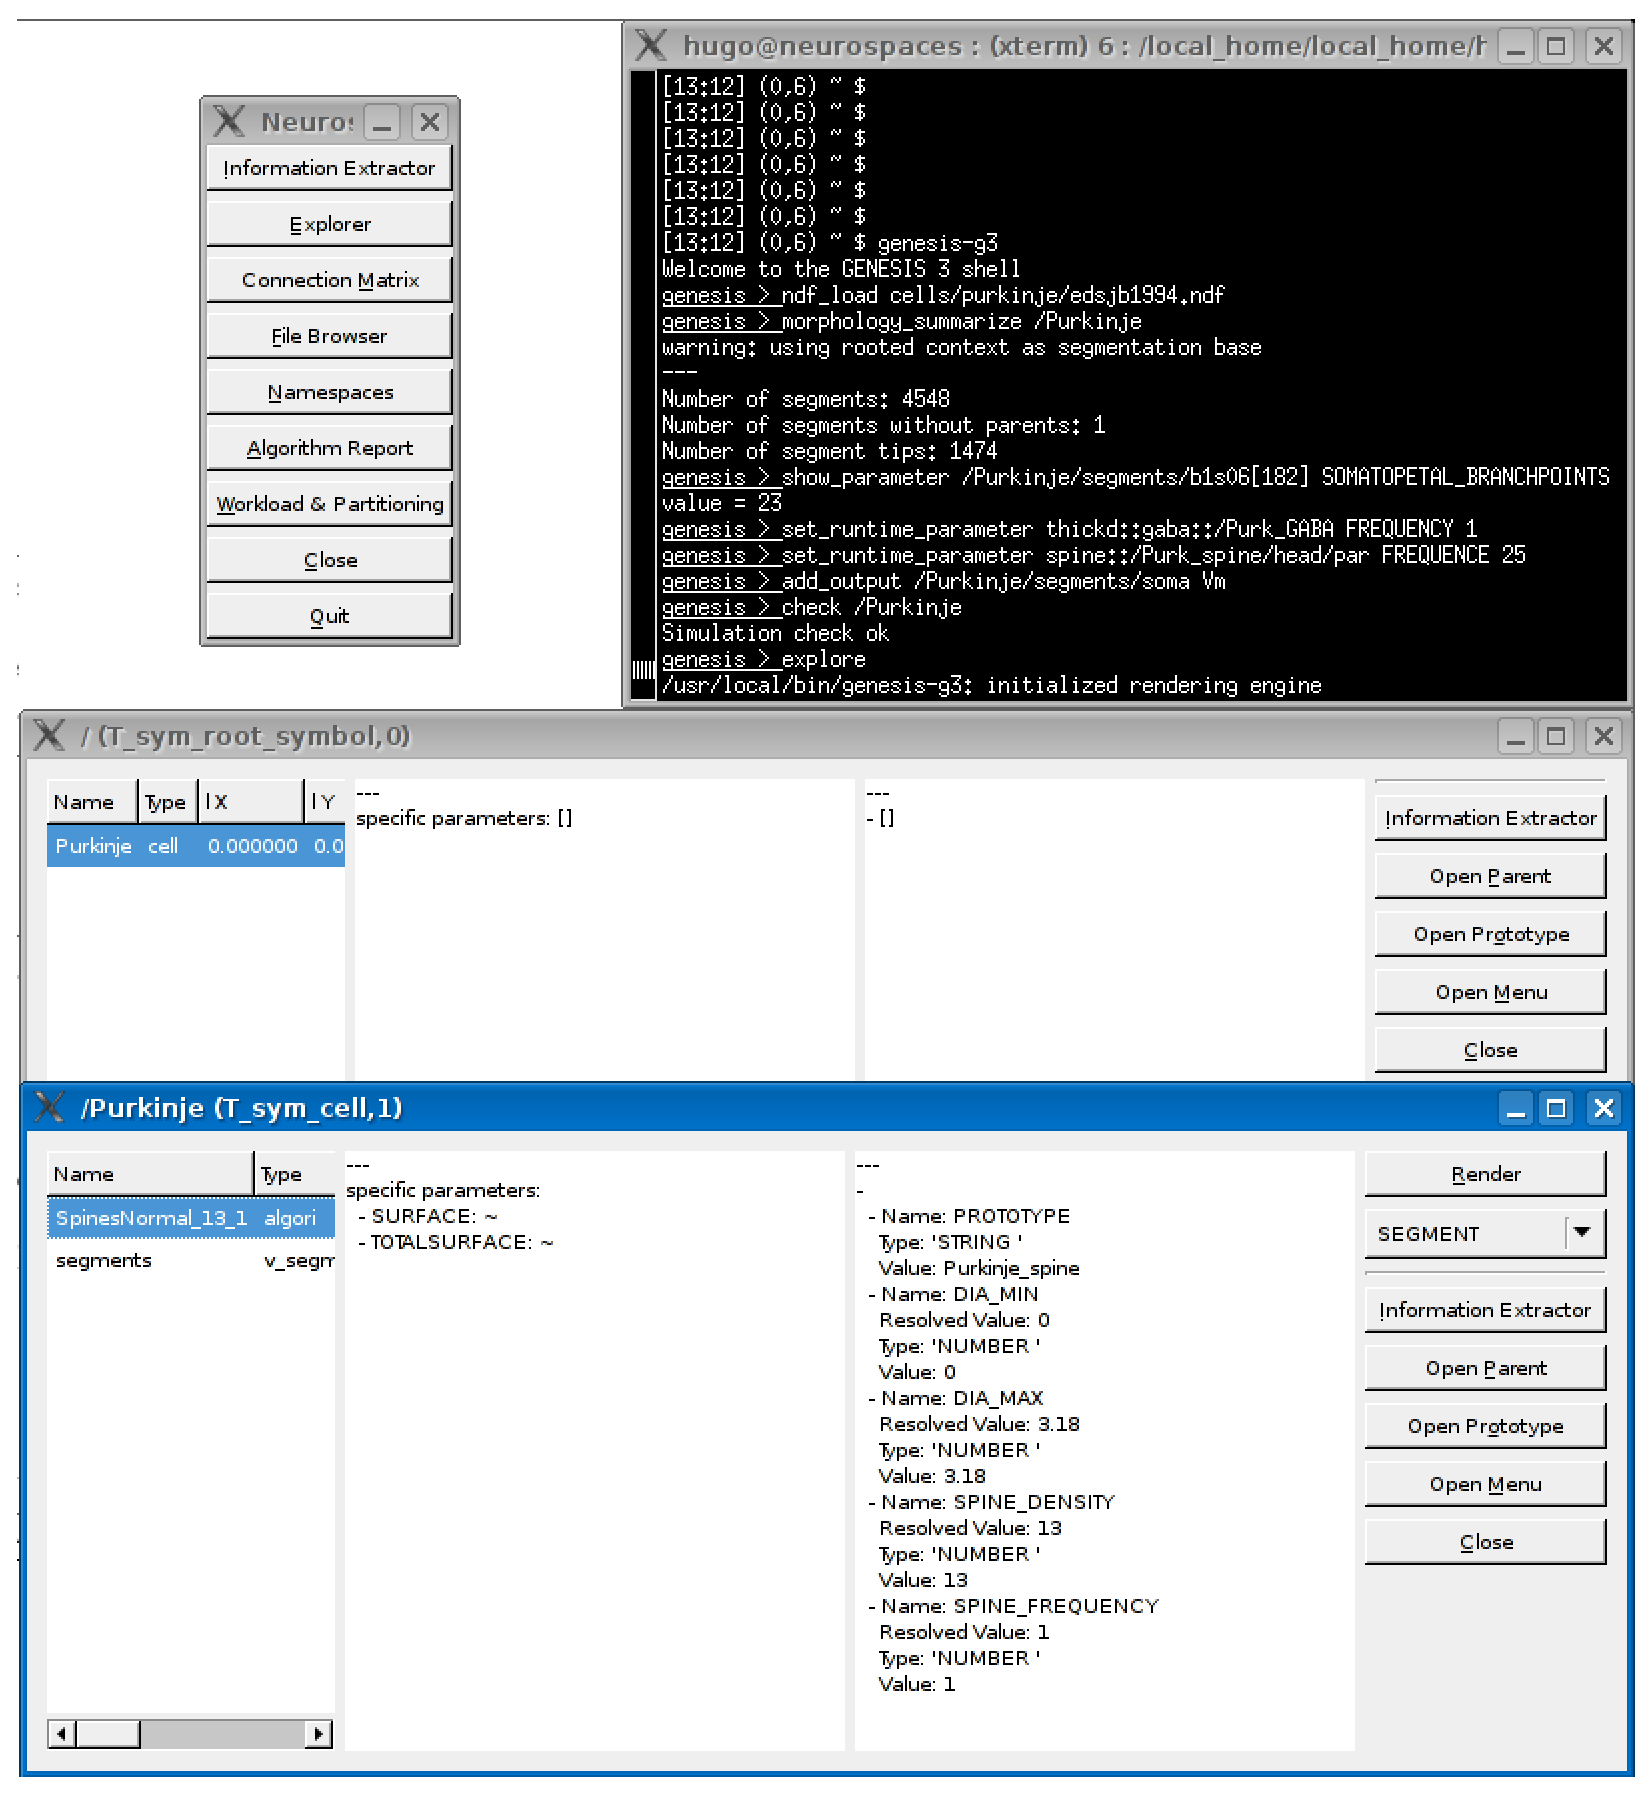
\includegraphics[width=4in]{figures/studio-screenshot.eps}
  \end{center}
  \caption{ {\bf Querying a model in GENESIS 3.0.} The {\bf Studio} is
    a G-3 simulator component that can
    be used to query the parameters of individual compartments in a
    multi-compartment model neuron. The {\bf Studio} also renders 3D
    morphology of dendrites and generates overviews of network models.
  }
  \label{fig:cbi-studio}
\end{figure}

Figure~\ref{fig:cbi-studio} shows sample output of running this
command.  Other capabilities of the {\bf Studio} include rendering
morphologies in three dimensions and generating overviews of network
models (not shown). 

%In the next section we explore some of the more
%graphical capabilities of G-3.

\subsection{Simple Scripting}
\label{ss-apens}

Python is a high-level scripting language that uses modules to group
related functions.  G-3 employs Python's module system to group the
functions that provide an interface to each of the simulator's
software components.
%G-3 scripting
%bindings use modules to separate interfaces for simple models with
%many default settings (e.g. to start a new research project) from more
%complicated interfaces that expose the full functionality of the
%simulator.
As an example, the G-3 Python module {\it nmc} contains functions to
simplify the storage of neuron models in computer memory.  The module
is a simple front-end to the {\bf Biology\,Model\,Container}.
Likewise, {\it Heccer} is a wrapper module for the {\bf Heccer}
component.  We note that Python bindings for {\bf DES} to facilitate network modelling are in development.

%Here we show a simple example of a high-level Python script that runs a simulation of a single cylindrical segment. It
%is defined by standard values for the parameters of membrane
%resistance ({\tt RM}), axial resistance ({\tt RA}), and membrane
%capacitance ({\tt CM}). (Note: This script
%  is written for clarity of presentation rather than compactness or
%  efficiency.)
%%\footnote{The solver requires {\tt RA} for all
%%  compartments.}
%Parameters are given by their specific values (in SI units) as
%commonly reported in the literature, instead of their actual values
%scaled to the compartment surface area as used by a mathematical
%solver \cite{cornelis04:_neuros_param_handl}. The script defines a
%Python function {\it run\_simulation} that will load and run a model when invoked from
%a system command line on an appropriately configured computer.  The script
%can also be imported into G-3 as a Python module, thus allowing access
%to this function.  For convenience, we call this Python module {\it
%  example}.
%
%\begin{verbatim}
%"""
%Comment: Python script running a simple model with G-3.
%"""
%from g3.nmc import ModelContainer
%
%def RunSimulation(simulationTime):
%    timeStep = 1e-5
%    
%#------------------------------------------------------------------------------
%# Create a model container with a neuron cell and a dendritic segment
%#------------------------------------------------------------------------------
%    my_nmc = ModelContainer()
%    my_cell = my_nmc.CreateCell("/cell")
%    my_segment = my_nmc.CreateSegment("/cell/soma")
%
%    my_segment.SetParameters(
%        {
%        "Vm_init": -0.0680,
%        "RM": 1.000,
%        "RA": 2.50,
%        "CM": 0.0164,
%        "ELEAK": -0.0800,
%        "DIA": 2e-05,
%        "LENGTH": 4.47e-05,
%        }
%        )
%
%# Apply current injection to the soma
%    my_segment.SetParameter("INJECT", 1e-9)
%
%#------------------------------------------------------------------------------
%# Create a Heccer for computing the neuron model stored by the model container.
%#------------------------------------------------------------------------------
%    from g3.heccer import Heccer
%    my_heccer = Heccer(name="/cell", model=my_nmc)
%    my_heccer.CompileAll()
%
%#----------------------------------------------------------------------------- 
%# Create an output object.
%#------------------------------------------------------------------------------
%    from g3.experiment.output import Output
%    my_output = Output("/tmp/output")
%
%#----------------------------------------------------------------------------- 
%# Link the output object to the address of the computed variable of interest.
%#------------------------------------------------------------------------------
%    my_output.AddOutput("output", my_heccer.GetAddress("/cell/soma", "Vm"))
%
%#----------------------------------------------------------------------------- 
%# Create an array of the objects that participate in the simulation.
%#------------------------------------------------------------------------------
%    schedulees = []
%
%    # schedule heccer
%    schedulees.append(my_heccer)
%    schedulees.append(my_output)
%
%#----------------------------------------------------------------------------- 
%# Advance all the particpating objects for the duration of the simulation.
%#------------------------------------------------------------------------------
%    currentTime = 0.0
%    while currentTime < simulationTime:
%        currentTime += timeStep
%
%        for schedulee in schedulees:
%            schedulee.Advance(currentTime)
%
%    my_heccer.Finish()
%    my_output.Finish()
%  
%#------------------------------------------------------------------------------
%# Main program executes a simulation of 0.5 seconds.
%# The if statement allows use of this file as an executable or as a library.
%#------------------------------------------------------------------------------
%
%if __name__ == '__main__':
%    RunSimulation(0.5)
%\end{verbatim}
%
%%# Second Example: use a wildcard to activate endogenous synapses (see text)
%%#    my_nmc.Query("setparameter spine::/Purk_spine/head/par 25")
%%#    my_nmc.Query("setparameter thickd::gaba::/Purk_GABA 1")

\subsection{Scripting Chemesis-3}

The following example, {\it cal1.ndf}, shows how to implement a G-2
Chemesis tutorial in G-3.  It creates a single compartment that
contains interaction between calcium and a buffer.

%, {\it cal2.g} creates a two
%compartment model with a dendrite and soma with an additional diffusion object
%for diffusion between the compartments

\begin{verbatim}
NEUROSPACES NDF
PUBLIC_MODELS
  KINETICS cal1
    PARAMETERS
      PARAMETER ( DIA = 24e-4 ),
      PARAMETER ( LENGTH = 24e-4 ),
    END PARAMETERS
    POOL somaCa
      BINDABLES OUTPUT concen END BINDABLES
      PARAMETERS
        PARAMETER ( concen_init = 0.001 ),
        PARAMETER ( "UNITS" = 1e-3 ),
      END PARAMETERS
    END POOL
    POOL somaCabuf
      BINDABLES OUTPUT concen END BINDABLES
      PARAMETERS
        PARAMETER ( concen_init = 0.003 ),
        PARAMETER ( "UNITS" = 1e-3 ),
      END PARAMETERS
    END POOL
    POOL somabuf
      BINDABLES OUTPUT concen END BINDABLES
      BINDINGS
        INPUT ../somaCabuf->concen,
      END BINDINGS
      PARAMETERS
        PARAMETER ( concen_init = 0.153 ),
        PARAMETER ( concen_total = 0.153 ),
      END PARAMETERS
    END POOL
    REACTION somacabufrxn
      BINDABLES INPUT concen, OUTPUT concen END BINDABLES
      BINDINGS
        INPUT ("substrate") ../somaCa->concen,
        INPUT ("substrate") ../somabuf->concen,
        INPUT ("product") ../somaCabuf->concen,
      END BINDINGS
      PARAMETERS
        PARAMETER ( FORWARD_RATE = 1e2 ),
        PARAMETER ( BACKWARD_RATE = 0.5 ),
      END PARAMETERS
    END REACTION
  END KINETICS
END PUBLIC_MODELS
\end{verbatim}

The length and diameter of the pools required to complete the model
take on their implicit default values of:
\begin{verbatim}
  PARAMETER ( DIA =  ..->DIA ),
  PARAMETER ( LENGTH =  ..->LENGTH ),
\end{verbatim}

The following commands illustrate how the {\bf G-Shell} and the {\bf Studio} may be employed
to load  {\it cal1.ndf} into the {\bf Biology\,Model\,Container} for exploration of this model:

\begin{verbatim}
  ndf_load chemesis/cal1.ndf
  explore
\end{verbatim}

%while, the {\bf G-Shell} command to run {\it cal1.ndf} and send output to
%a file is:
%
%\begin{verbatim}
%  genesis > run /cal1 2
%\end{verbatim}

\section{Results}

\subsection{Addressing Scheme Algorithm}

The different solvers contributing to a multi-scale simulation can
hold equivalent variables.  These variables exist because two or more
physical processes of the model have been bound using the {\tt
  BINDINGS} in an NDF file.  During a simulation, {\it the addressing
  scheme algorithm} enables the {\bf Solvers} and the {\bf
  Communication\,Infrastructure} to relate any equivalent variables
these components contain.  As this happens during a simulation, {\it
  the addressing scheme algorithm} must be highly optimized to
maximize run-time performance.

The information required to identify a variable (and hence its
address) is obtained from the model stored in the {\bf
  Biology\,Model\,Container}. To achieve this, the {\bf
  Biology\,Model\,Container} defines an addressing scheme that is able
to refer to or `address' the variables of every model component.
These addresses provide the `hooks' for attaching ``experimental
protocols'' (e.g. stimulus and output specifications) to the {\bf
  Solvers}.  The addressing scheme is not necessarily dependent on the
NDF format. It is more general in the sense that it provides an
interface to external software applications such as GUIs and
databases.

In G-3, the algorithm for taking the simulation-time address of a
computed variable consists of three steps.

\paragraph{Step 1} Translates NDF names to a hierarchical namespace.
The scheme defines a symbolic syntax for the hierarchical addressing
of model components and their parameters and variables.  The syntax
allows a user to express the address of a variable, for example, the
address of the $\mathrm{Ca}^{2+}$ concentration in a segment, with the
name `soma':
\begin{verbatim}
  /soma/Ca->conc
\end{verbatim}

\paragraph{Step 2} The second step is the translation of symbolic
references to IDs and is implemented in the {\bf
  Biology\,Model\,Container}. There, the hierarchical namespace
(created during step 1) is translated to simulation wide unique tuples
of the form [integer, type].  The integer identifies the physical
process and the type identifies the variable containing the
concentration level.

%This constructs an interface that identifies the solver instance
%associated with each physical process (here the $\mathrm{Ca}^{2+}$
%pool).

%This translation is only required during simulation construction, and
%not during simulation run-time.  Once constructed, the tuples are
%independent of the {\bf Biology\,Model\,Container}.

\paragraph{Step 3} The third step of the addressing algorithm
translates [integer, type] tuples to tuples of the form [solver
instance, internal ID].  This step is low-level and implemented in the
{\bf Solvers}.

After this step of the algorithm, an interface has been defined that enables
the communication port of the solver that attaches to the given
variables to be obtained.  This interface allows a solver instance
internal ID to be obtained for directly addressing the variable.

The addressing scheme algorithm allows {\bf Solvers} to communicate
through the tuples [solver instance, internal ID].  The advantage is
that the {\bf Biology\,Model\,Container} does not have to be in memory
during simulation run-time.  This removes any requirement for
expensive computation on symbolic or hierarchical addresses during
simulation run-time.

Software may choose to implement the interface between solvers using
memory pointers for maximum efficiency, or, alternatively, using a
low-level function that reads and writes the variable.  This feature
may be useful in a parallel implementation for example.

%  However it may be required during
%simulation run-time, depending on the model and stimulus
%paradigm\marginpar{I don't see when?}.


\subsection{DES: Action Potential Propagation Abstraction}

The Discrete Event System ({\bf DES}) is used for the abstract
modelling of action potentials, a functionality required for the
running of network simulations.  Action potentials generated at the
soma of one neuron are translated to a discrete event that is
delivered to the post-synaptic targets of a connected neuron.  {\bf
  DES} also associates `secondary' data with a connection, for
example, propagation delay, synaptic weight, or other data specific
for the model.

Internally, {\bf DES} contains two subcomponents, one for event
distribution that contains a connectivity matrix, the second for event
queuing.  In the CBI architecture, the {\bf DES} event queuer is a
separate solver that simulates action potential propagation in an
efficient way.  The {\bf DES} event distributor provides communication
between the solvers during the simulation.

The separation of the discrete event functionality from the rest of
the simulator facilitates customization for the modeling of
sophisticated learning rules, especially those related to STDP,
diffusion, and spillover \cite{roberts02:_spike, nowotny03:_enhan}.

\subsection{Multi-Scale Network Modeling}

Network modelling was previously possible in
G-2 \cite{cornelis02:_tutor}.  To simulate networks of cells the user
must manually initialize the numerical solver of G-2 for
every cell in the network.  Careful G-2 script coding was required to
prevent memory exhaustion errors.  The complexity of the G-2 procedural scripts contrasts with the simplicity of the configuration of the G-3 addressing scheme given below.


The {\bf SSP} software component defines several software regression
tests with network models.  One of the simplest network models used in
this test has a `source' neuron that delivers a spike to two
`target' neurons during the simulation .

To simulate this simple network, the simulation configuration has to
associate each neuron model in the {\bf Model\,Container} with {\bf
  Heccer}.  This association will then create a {\bf Heccer} instance
before the simulation starts.  As with G-2, in G-3 this is currently a manual
operation.
%In G-3 multi-scale network modelling of individual neurons requires a
%{\bf Heccer} instance for each neuron.
However, the integration of the user workflow into G-3 defines
the scope of user actions and in the case of network modeling, allows
the {\bf Heccer} instances, once created, to share internal data
structures as required, thereby transparently reducing overall memory consumption.

In G-3 the action potential propagation through the fibers of a
projection is simulated by the event queuing component of {\bf DES}.
The {\bf G-Shell} syntax is:
\begin{verbatim}
  ndf_load tests/networks/spiker4.ndf
  solverset "/network/target1 => heccer"
  solverset "/network/target2 => heccer"
  solverset "/network/source => heccer"
  solverset "/network/projection => des"
\end{verbatim}

%Internally, the {\bf G-Shell} translates these statements to their
%equivalent {\bf SSP} syntax:
%\begin{verbatim}
%  { modelname => "/network/target1",
%    solverclass => "heccer", },
%  { modelname => "/network/target2",
%    solverclass => "heccer", },
%  { modelname => "/network/source",
%    solverclass => "heccer", },
%  { modelname => "/network/projection1",
%    solverclass => "des", },
%\end{verbatim}


\subsection{Multi-Scale Scripting}

In  a typical multi-scale model
different numerical solution methods are required to solve the different
types of mathematical equations associated with the different scales of the
model.  In G-3 the cable equation and ion currents are numerically solved with
implicit Crank-Nicolson integration using {\bf Heccer}.  Calcium models are numerically solved with {\bf Chemesis-3}.
The association between a given model and its {\bf Solvers} can be configured by the user.
%Under planned extensions to the G-shell syntax, the correct syntax
%for a loaded single neuron model with name "/Purkinje" would be:
For example to associate the model named ``/Purkinje'' with the solver {\bf heccer}, the command is:
\begin{verbatim}
  solverset "/Purkinje => heccer"
\end{verbatim}

To use {\bf Chemesis-3} to simulate a complex network model of
biochemical pathways, here called {\it cal1}, a user would type in the
G-3 shell:

\begin{verbatim}
  solverset "/cal1 => chemesis3"
\end{verbatim}

In the case where a network of biochemical pathways is defined inside a
single neuron model, a user would have to type two commands with
wildcards to associate the correct solver with each component of the
model, for example:

\begin{verbatim}
  solverset "/**/cal1 => chemesis3"
  solverset "/Purkinje/**[!cal1] => heccer"
\end{verbatim}

%In later versions of G-3 these rules will be built in but still allow
%the user to select a different method of solution for different
%components of a model.


\section{Discusion}

Simulation provides a framework to organize our understanding of biological systems. Historically, the development of neuronal simulation software for the construction of morphologically detailed neuron models and small networks has been instigated by research projects that specifically addressed complementary technical and scientific questions \cite{Moore:2010vn}. These software systems have been both highly successful and continue to grow in complexity through cycles of research project extension. However, after more than twenty years of extending their functionality, usually by the direct incorporation of source code into the core of the simulator (typically comprising a single solver), code structures have become so complicated that it is increasingly difficult, if not impossible, to easily continue extension of simulator functionality. Ultimately, the resulting stand-alone applications become `monolithic'. In these conditions it is a considerable challenge for a neuroscientist lacking the necessary mathematical and computational skills to extend a model. In practice, the complexity and monolithic nature of the software results in a non-scalable software architecture \cite{jaeger02:_comput_neuros_realis_model_exper}.

At the core of the problem is the lack of distinction in many contemporary simulators made between biological data, numerical data, and control operations during the software architecture development stage of simulator design. The majority of such simulators remain primarily focused on the biological and mathematical aspects of a model. As they do not respect all three of Marr's levels, i.e. the third of Marr's levels (``hardware'' implementation) is not addressed during software design, the complexity of multi-scale simulation is greatly increased. 

We note that just as the `hardware' of a biological system should be accounted for in the cognitive process of model development, so must it be accounted for during the simulation of the model. In a simulator this can be achieved by the software architecture and its organization of simulator functionality. Making the cognitive model concordant with simulator functionality removes many of the problematic aspects of multi-scale modeling.  

It has previously been proposed that \cite{Sejnowski:1988fk}: (1) because of the the many different structural levels of organization and the fact that models rarely span more than two levels, a more comprehensive understanding of a system requires many different types of model, and (2) intermediate level models must necessarily simplify with respect to the structural properties of lower level elements. We consider this view to be based on the difficulty of employing a monolithic simulator to address a multi-level problem.

To clarify these issues, we turn to a discussion in \cite{Heylighen:2006vn}. Systems theory shows that regardless of the number of scales used to conceptualize a system, it is not possible to know whether the system has been completely conceptualized. This is a consequence of changing scales as when this occurs it adds, deletes, and reconfigures patterns that are the content of the associated conceptualizations. There is no way to know or learn that all patterns have been conceptualized at one or more scales, as completeness is not possible. Nevertheless, the use of multiple scales of conceptualization provides a way to asymptotically approach completeness.
 
However, as \cite{Heylighen:2006vn} continues, at any scale of conceptualization, properties are always aggregated at least as simple objects. Thus, a system at any scale of conceptualization is an approximation or loose congruence of the actual system. This is not an `abstraction' of the system as that means leaving things out of a model with the understanding that what is absent can always be reinserted. What is ``left out'' of a scale specific conceptualization of a system are patterns (simple objects, relationships, and their aggregations) that might be available at other scales. Such patterns cannot be returned to a scale specific approximation of a system, regardless of resolution or field of view. This means that `missing' content has no place in a conceptualization at a given scale as it was never available in the first place.

According to principles of systems theoretic analysis (see \cite{Bertalanffy:1973zr,Heylighen:2006vn}), it is clear there are numerous phenomenological approaches to the development of multi-scale models suited to the transformation of a mental model into a computational simulation. We resolve this problem by expansion of the cognitive workflow as illustrated in Figure \ref{fig:mental-model-simulation-path}.

The cognitive workflow is an adaption of a previously described user workflow that organizes the sequence of necessary steps typically employed by a person in developing a computational model and employing simulation to generate data for subsequent analysis \cite{10.1371/journal.pone.0028956}. In this sense it is a depiction of a sequence of operations, declared as the work of a person or a group of persons (Belhajjame et al., 2002). Similarly, the cognitive workflow describes the process whereby an abstraction is transformed into an implementation by the conversion of a mental model into a simulation. This is made possible due to the recent reconfiguration of the GENESIS simulator. 

The reconfiguration complied with the CBI architecture which is based on a separation of concerns. It partitions data and control functions from software layering that separates high level biological data from low level mathematical operations. The immediate benefit of this partitioning (see \cite{10.1371/journal.pone.0028956} for details), is transparent support of multi-scale simulation.

The approach is based on the implementation of a model for simulation being contained by a single software entity (here a single {\bf Biology\,Model\,Container}). This single entity interfaces with the multiple solvers required to address the different scales of a model, but it is only needed during the construction of the model. A communication infrastructure enables communication at run-time between these solvers and thus across different levels of a simulation. In this paradigm, the requirement for multiple models is removed by implementation of multiple solvers. As a consequence, simplification of intermediate models with respect to lower levels as proposed by \cite{Sejnowski:1988fk} may be eliminated. 

%, but ought to attempt to incorporate as many of the given level's functional properties as actually exist in the higher level's computational tasks. This approach has led to the development of both realistic brain models containing considerable biological detail and simplifying brain models that `abstract' both structural and functional principles, although any given model may have features of both.

%The CBI architecture was designed to address this situation, thereby enabling transparent simulator extensibility and as a consequence the implicit implementation of multi-scale modelling.

%The core of these problem is the 
%lack of distinction in the majority of contemporary simulators between biological data, numerical data, and control operations during the design and development of a simulator. The majority of contemporary simulators remain primarily focused on these biological and mathematical aspects of a model. As they do not respect all three of Marr's levels, the complexity of multi-scale simulation is greatly increased. 

To this end, G-3 supports the construction of multi-scale network and system
models based on realistic neuronal components.  In support of
this function, the G-3 {\bf Biology\,Model\,Container} applies specific algorithms to
instantiate systems level connectivity models and convert them to
mathematical representations. This relieves the mathematical solvers from
the algorithmic pressures typical for rich heterogeneous model structures.  At the
same time, intermediate simulation system modules, already
described as the mechanism used to link {\bf Chemesis-3} and linear
cable solvers, are used to share values and functions between
larger scale network simulations and lower scale models.

From a technical point of view, the incorporation of simulation
modules that specifically involve spatial dimensions is, in principle,
much more difficult than the integration of biochemical kinetic
models. In fact the accurate representation of space and time for
multi-scale simulations is an open research area.  However, the
explicit provision of software modules for the intermediary
representation of solved variables allows the comparison and evaluation of
different methods of scale-linking, for instance by comparing
different resolutions of a fixed grid with adaptive grid intermediary
representations \cite{MO:2009bh}. In effect, this allows
the use of multi-scale G-3 models as a framework to compare different
technical strategies.

The developing paradigm of multi-scale modelling reported here
enables the generation of a taxonomy of models in computational neurobiology
based on both the biological scale of a model and the level of detail
it aims to represent. By accounting for each of the levels proposed in \cite{Marr:19821kx} during development of a simulator, it is possible to transparently resolve many of the technical and conceptual issues currently surrounding the successful simulation of multi-scale models.

%Ignoring these distinctions results in `collapse' of the cognitive workflow into a single node located at the last step of the cognitive workflow. This convergence is illustrated in Figure \ref{fig:mental-model-simulation-part}. The figure shows that in a monolithic software system high convergence allows only a single (monolithic) software component to exist. This suggests that in the absence of a clean separation of concerns, otherwise prohibited diagonal interactions are introduced between the Control/Data and High/Low software axes defined in Figure \ref{fig:cbi-architecture-simple}.
%
%\begin{figure}[h!t]
%  \begin{center}
%    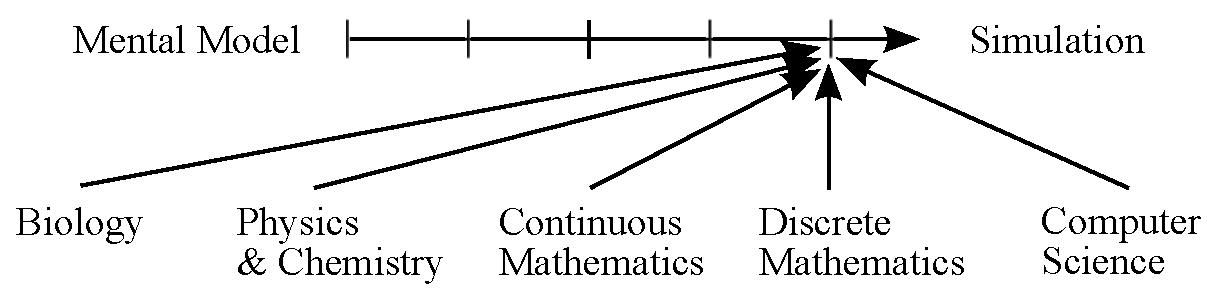
\includegraphics[width=4in]{figures/NS-abstraction-implementation-part.eps}
%  \end{center}
%  \caption{ {\bf Cognitive Workflow of Monolithic Software.} }
%  \label{fig:mental-model-simulation-part}
%\end{figure}
 
%Figure \ref{fig:mental-model-simulation-path} illustrates a selection of some of the possible steps, levels, and components of the cognitive workflow we employ here. Interestingly, two possible multi-scale models have been in widespread use but not generally recognized for their multi-scale characteristics: (1) Biologically inspired, e.g. a model is specified as a network and a population of detailed channel models, and (2) Mathematically inspired, e.g. use continuous cable equations to model a neuron, discrete event models for axonal propagation, and Hodgkin-Huxley equations for the channels.

 % Contrast this with \cite{ray08:_pymoos}

%- Summary.
%
%- Parts of the multiscale grant.

%\begin{figure}[ht]
%  \begin{center}
%    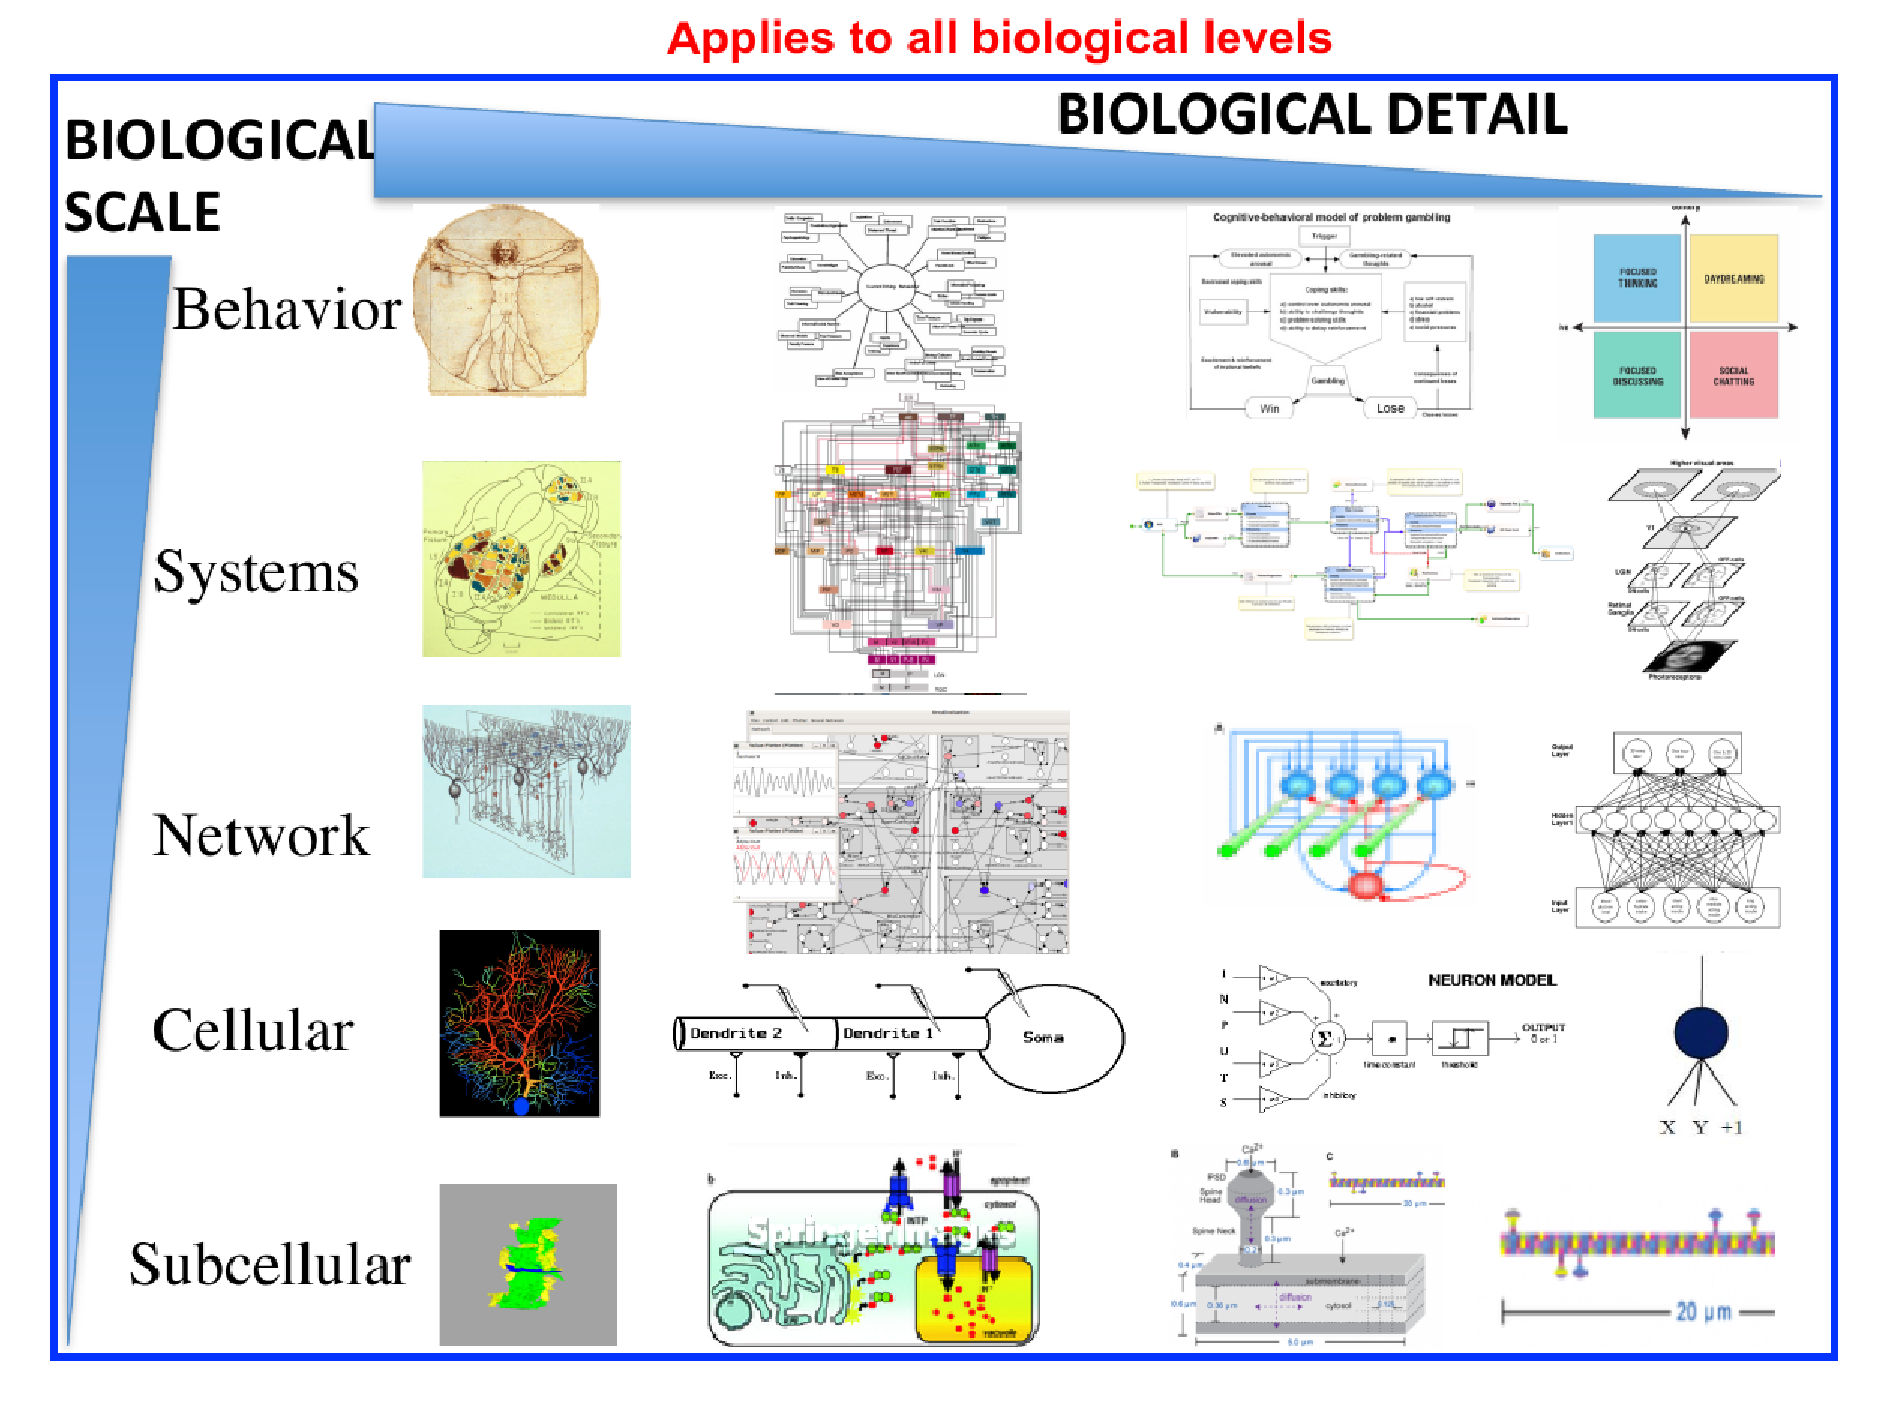
\includegraphics[width=4in]{figures/multi-scale-taxonomy.eps}
%  \end{center}
%  \caption{ {\bf Taxonomy of Multi-scale Models.} }
%  \label{fig:multi-scale-taxonomy}
%\end{figure}

%Incorporate two types of 3-D Monte Carlo-based techniques for modeling
%reaction/diffusion kinetics. Specifically, Dr. Avrama Blackwell will
%work with the G-3 development team to implement NeuroRD (Oliveira et
%al., 2010), a computationally efficient approximate Monte Carlo
%approach to modeling reaction-diffusion systems.
%
%In addition, the G-3 development team will work with Dr. Yoshi Kubota
%to incorporate 'CDS' (Cellular Dynamics Simulator:
%http://nba.uth.tmc.edu/cds/) a precise particle-based Monte Carlo
%simulator specifically supporting the modeling of Ca2+ binding and
%diffusion dynamics within biochemical networks (Byrne et al. 2010;
%Kubota and Waxham 2011). CDS is based on the event-driven first
%passage time algorithm (Byrne et al. 2010) and is designed to serve as
%a flexible platform for multi-scale hybrid algorithms.  For this
%reason, the CDS algorithm can be directly combined with any
%deterministic ODE/PDE (Reaction-Diffusion Equation) solvers (e.g.,
%V-Cell used in Hernjak et al. 2005) including those already included
%in G-3.  High-resolution cellular morphology including that of
%dendritic spines can be directly transported to CDS allowing
%electro-diffusion to be simulated by both deterministic (as in
%Lopreore et al. 2008) as well as particle-based 3-D stochastic
%methods.
%
%This will allow us to compare different simulation algorithms for Ca2+
%binding diffusion, voltage clamp, and biochemical network within the
%same platform and will help derive and validate simplified macroscopic
%(biochemical) synaptic rules relevant to the objectives of Specific
%Aim 2.

%\subsection{additional references}
%
%DeSchutter, E., and Bower, J.M. (1994)  An Active Membrane Model of the
%Cerebellar Purkinje Cell: I simulation of current clamps in slice   J.
%Neurophysiol.  71:375-400.
%
%Kotaleski, J. H., Plenz, D. and Blackwell, K. T. (2006) Using potassium
%currents to solve signal-to-noise problems in inhibitory feedforward
%networks of the striatum. J. Neurophysiol.  95: 331-341.
%
%- dave's chapter
%
%- visual interface to neuron (see Jim's review invitation)
%
%- numerical solvers, see Andrew Davison's email.


%\begin{figure}[h]
%  \centering
%   
\includegraphics[scale=0.5]{figures/dummyfig.eps}
%\caption{{\bf A Dummy Figure:} Example of \LaTeX\,\,\,code to incorporate a figure into documentation.}
%  \label{fig:df-2}
%\end{figure}

\section*{Acknowledgements}

Hugo Cornelis was partially supported by the CREA Financing program
(CREA/07/027) of the K.U.Leuven, Belgium, EU.  Both Hugo Cornelis,
Allan D. Coop were partially supported by NIH grant 5 R01 NS049288-08
to James M. Bower.  We thank the Australian and Belgian Governments
for their support of employable people.

Armando L. Rodriguez and David Beeman, were supported by NIH grant 5
R01 NS049288-08 and 3 R01 NS049288-06S1 to James M.  Bower.

We also thank the Computational Biology Initiative at UTSA
(http://www.cbi.utsa.edu) for their support when installing, using,
and updating G-3 on their computers.


\newpage

\bibliographystyle{plain}
\bibliography{../tex/bib/g3-refs.bib}

\end{document}
